%\documentclass[12pt,report]{jsbook}	%片面印刷
\documentclass[12pt]{jsbook}	%両面印刷

%\bibliographystyle{jplain}


\usepackage[dvipdfmx]{graphicx}
\usepackage[dvipdfmx]{color}
\usepackage{amsmath}
\usepackage{amssymb}
\usepackage{cite}
\usepackage{mathrsfs}
\usepackage{color}

\usepackage{latexsym}
\usepackage{wrapfig}
\pagestyle{plain}
\usepackage{fancybox}
\usepackage{bm}
\usepackage{booktabs}
\usepackage{mediabb}

\numberwithin{equation}{section}

\newcommand{\divergence}{\mathrm{div}\,}  %ダイバージェンス
\newcommand{\grad}{\mathrm{grad}\,}  %グラディエント
\newcommand{\rot}{\mathrm{rot}\,}  %ローテーション

\renewcommand{\baselinestretch}{1.1}	%行間の調整

%chapterの文字サイズ、位置の調整-------------------------------
\makeatletter%% プリアンブルで定義する場合は必須

\def\@makechapterhead#1{\hbox{}%
  \vskip2\Cvs
  {\parindent\z@
  \raggedright% オリジナルの定義(左揃え)
%   \centering% 中央揃え
%  \raggedleft% 右揃え
   \reset@font\huge\bfseries
   \ifnum \c@secnumdepth >\m@ne
     \setlength\@tempdima{\linewidth}%
     \vtop{\hsize\@tempdima%
         \@chapapp\thechapter\@chappos\\%
     #1}%
   \else
     #1\relax
   \fi}\nobreak\vskip3\Cvs}

\def\@makeschapterhead#1{\hbox{}%
  \vskip2\Cvs
  {\parindent\z@
  \raggedright% オリジナルの定義(左揃え)
%   \centering% 中央揃え
%  \raggedleft% 右揃え
   \reset@font\huge\bfseries
   \setlength\@tempdima{\linewidth}%
   \vtop{\hsize\@tempdima#1}}\vskip3\Cvs}

\makeatother%% プリアンブルで定義する場合は必須
%------------------------------------------------------------

%\bibliographystyle{jplain}

%-------------------------------------
%\documentclass[12pt]{jreport}

%\usepackage{graphicx}
%\usepackage{bm} 
%\usepackage{amsmath,amsthm,amssymb}
%\usepackage{epic, eepic}


%\pagestyle{empty}

%\setlength{\textwidth}{14.5cm}
%\setlength{\textheight}{23cm}
%\setlength{\oddsidemargin}{0.75cm}
%\setlength{\topmargin}{-6mm}
%\setlength{\headsep}{35pt}

%\renewcommand{\baselinestretch}{1.07}

%\setlength{\oddsidemargin}{-5mm}
%\setlength{\topmargin}{-10mm}
%\setlength{\textheight}{18.3cm}%両面印刷の時必要
%\def\baselinestretch{1.5}
%\setlength{\textwidth}{170mm}
%\setlength{\marginparsep}{-5mm}
%\setlength{\marginparwidth}{-5mm}


%\textwidth=15cm
%\textheight=240mm
%\oddsidemargin=3mm
%\topmargin=-6mm
%\headheight=8mm
%\headsep=0mm
%\footskip=15mm
%\marginparwidth=0mm
%\marginparpush=0mm
%\marginparsep=0mm

%\setcounter{topnumber}{100}
%\setcounter{bottomnumber}{100}
%\setcounter{totalnumber}{100}
%\renewcommand{\topfraction}{1.0}
%\renewcommand{\bottomfraction}{1.0}
%\renewcommand{\textfraction}{0.0}
%\renewcommand{\floatpagefraction}{0.0}


%\setcounter{secnumdepth}{2}
%\setcounter{tocdepth}{2}
%\renewcommand{\thepart}{\arabic{part}}

%\makeatletter
%\renewcommand{\thesection}{\thepart.\arabic{section}}
%\@addtoreset{section}{part}
%\renewcommand{\theequation}{\thepart.\arabic{equation}}
%\@addtoreset{figure}{part}
%\renewcommand{\thefigure}{\thepart.\arabic{figure}}
%\@addtoreset{equation}{part}
%\renewcommand{\thetable}{\thepart.\arabic{table}}
%\@addtoreset{table}{part}
%\makeatother

%\renewcommand{\figurename}{Fig.~}
%\renewcommand{\tablename}{Table~}

%\includeonly{part2,part3,part4,part5,reference}






%平行
%\def\para{%
%\setlength{\unitlength}{1pt}%
%\thinlines %
%\begin{picture}(12, 12)%
%\put(0,0){/}
%\put(2,0){/}
%\end{picture}%
%}%

%-------------------------------------



\begin{document}


\begin{titlepage}
\noindent
\Large{
修士論文
\hspace*{45mm}
2018(平成30)年度
}
\\
\\
\Large{
論文題目
}
\\
\huge{\center{
磁性体/酸化物及び有機物ヘテロ構造\\
におけるスピンダイナミクスの研究

	}
}
\vspace{3mm}
\begin{center}\Large 
Spin Dynamics in Magnetic Materials/Oxide \\
and Organic Materials Heterostructures
\end{center}

\vspace*{13mm}
\Large{
	\center{
慶應義塾大学
\\
理工学研究科
\\
	}
}
\vspace*{6mm}
\Large{
	\center{
学籍番号\hspace*{5mm} 81612890 \hspace*{10mm}白怜士
\\
	}
}
\vspace*{3mm}
\Large{
	\center{
指導教員\hspace*{10mm} 安藤和也 \hspace*{2mm}准教授
\\
	}
}
\vspace*{3mm}
\Large{
	\center{
慶應義塾大学
\\
2018年2月
\\
	}
}
\end{titlepage}


\pagenumbering{roman}
%\pagestyle{empty}
%\tableofcontents
\setcounter{tocdepth}{2}\tableofcontents
\clearpage
%\pagestyle{plain}
\pagestyle{headings}%ヘッダー
\setcounter{page}{1}
\pagenumbering{arabic}




\chapter{序論}\label{chap:intro}

%\section{スピントロニクスとスピン流物理}


%電子とは負の電荷を持ち,固体物理の様々な特性を支配する基本粒子である.この電荷という内部自由度に加え,電子は角運動量という内部自由度も持つ.この角運動量は古典的に見れば電子がスピンしていることに対応しており,スピンと呼ばれる.このスピンは電子の相対論的量子力学におけるDirac方程式より導かれ,また磁性の起源ともなっている.

%従来のエレクトロニクスは電子における電荷の自由度のみに注目して発展を遂げた.しかし,電子にはスピンという.

身の回りを見回してみると家電製品や通信機器など多くのものがエレクトロニクスによって生み出されたものだと気づく.今の世界でエレクトロニクスはなくてはならない技術となっている.しかしエレクトロニクスは電子の電荷を利用することで展開している分野であり電子の持つもう一つの自由度,スピンを無視している.ここでスピンも電荷も利用しようとする学問がスピントロニクスである.スピンと電子の相互作用はナノスケールの長さで現れるため\cite{maekawa2002spin},1990年代におけるナノテクノロジーの大きな進歩がスピントロニクスの幕を上げたと言っても過言ではない.
スピントロニクスはスピンと電荷を組み合わせることによって革新的なデバイス機能を創り出そうとする分野である\cite{prinz1998magnetoelectronics,vzutic2004spintronics,wolf2001spintronics}.その発展は1988年における巨大磁気抵抗(GMR)の発見\cite{baibich1988giant,binasch1989enhanced}によって始まった.巨大磁気抵抗効果はGMR素子としてハードディスクドライブの磁気ヘッドなどに応用されていて,これは最初に成功したスピンデバイスとみなされている.
スピントロニクスの基本的な考え方は,今まで電子のスピンを無視して利用してきた電流に代わって,スピン分極した電子の流れであるスピン流を巧みに操るというものである.電荷に加えてスピンの自由度も考慮に入れると,今までは見えなかった電子の持つ効果や機能性が現れる.その一つが磁場を介さない磁化制御である.スピン流と磁化の相互作用はまだ解明されていない部分が大きいが,近年スピン流が磁化に与えるトルクの大きさを見積もる報告がされている\cite{hayashi2014quantitative,yang2014platinum}.本研究では,金属の界面に影響を与える自己組織化単分子膜(self assembled monolayer : SAM)という有機分子膜\cite{de2005tuning,love2005self,xu2014regulating}を用いて常磁性金属の表面状態を変化させ,そのときのスピン流によるトルクの変化を調べた.この研究によりスピン流によるトルクと金属表面との結びつきについて理解が深まるだけでなく,スピントロニクスの発展に寄与することが期待される.
本章ではまず磁化の運動方程式としてLandau-Lifshitz-Gilbert(LLG)方程式を導入する.そしてスピン流およびスピン蓄積を説明し,それらと磁化の相互作用として現れるスピン軌道トルクを定義する.

%\section{スピントロニクスと磁化制御}


%スピン流は,薄膜などの磁気構造に流すことで局所的な磁気電子と直接相互作用を引き起こせるため,磁化をコントロールする効果的な方法として注目を集めている.
%電気的に磁化をコントロールしている応用のひとつとして,商業的に利用されているSTT(spin transfer torque) MTJ(magnetic tunnel junction)メモリである.
%STTでは,磁化方向を固定された強磁性体層(固定層)に垂直に流れた電子はその磁化方向にスピン分極する.このスピン流は絶縁体を超えて,隣の強磁性体層にトルクを与え,磁化の方向を決めることができる.
%STTではスピン流のスピン分極を固定層によって誘起しているが,その代わり常磁性体/強磁性体の薄膜構造に面内方向へ電流を流したときに見られるスピン軌道相互作用を利用する方法がある.
\section{スピンと磁化ダイナミクス}
本節ではまず磁気モーメントのダイナミクスについての運動方程式を量子力学に導く.次にそれを磁化についての運動方程式に拡張し現象論的に緩和項を取り入れたLandau-Lifshitz-Gilbert(LLG)方程式について述べる.
\subsection{スピンについての運動方程式}
磁石の持つ磁性はほとんど電子のスピン角運動量によるものである.量子力学によると,スピン角運動量$\bm{s}$は磁気モーメント$\bm{\mu}$と比例関係にあり,
\begin{equation}
\bm{\mu} = -\gamma\bm{s}
\label{eq:mudef}
\end{equation}
と書ける.このときの比例定数$\gamma$は磁気回転比と呼ばれている.
これから磁化ダイナミクスを考える上でのスタートとして,この磁気モーメントが有効磁場$\bm{H_{0}}$の下にあるときの運動方程式を考える.$\bm{\mu}$と$\bm{H_{0}}$の間に両者を平行にするような相互作用を導入し,そのHamiltonianを次のように表す.

\begin{equation}
\sl{H} = -\bm{\mu}\cdot\mu_{0}\bm{H_{0}} = \gamma\mu_{0}\bm{s}\cdot\bm{H_{0}}
\label{eq:hamil1}
\end{equation}
ただし$\mu_{0}$は真空の透磁率である.

ここで,昇降演算子
\begin{equation}
\bm{\sigma_{+}} = \bm{\sigma_{x}} + \bf{i}\bm{\sigma_{y}}, \ \ 
\bm{\sigma_{-}} = \bm{\sigma_{x}} - \bf{i}\bm{\sigma_{y}}
\end{equation}
\begin{equation}
\therefore \bm{\sigma_{x}} = \frac{1}{2}(\bm{\sigma_{+}} + \bm{\sigma_{-}}), \ 
\bm{\sigma_{y}} =  \frac{1}{2\bf{i}}(\bm{\sigma_{+}} - \bm{\sigma_{-}})
\label{eq:sigmai}
\end{equation}
をPauli行列を用いてスピノル表示すると($\frac{\hbar}{2}\bm{\sigma} := \bm{s}$),
\begin{equation}
\bm{\sigma_{+}} \doteq \left(
\begin{array}{cc}
0 & 1\\
0 & 0
\end{array}
\right),\ 
\bm{\sigma_{-}} \doteq \left(
\begin{array}{cc}
0 & 0\\
1 & 0
\end{array}
\right)
\end{equation}
と表せ,$|\uparrow\rangle$,$\langle\downarrow|$に作用させると,
\begin{equation}
\bm{\sigma_{+}}|\uparrow\rangle = 0,\ \ 
\bm{\sigma_{+}}|\downarrow\rangle = |\uparrow\rangle,\ \ 
\bm{\sigma_{-}}|\uparrow\rangle = |\downarrow\rangle,\ \ 
\bm{\sigma_{-}}|\downarrow\rangle = 0
\end{equation}
となる.
一定の外部磁場$\bm{H_{0}}$が印加されているスピン状態のエネルギーは式(\ref{eq:hamil1})から,$\mp\gamma\mu_{0}\bm{H_{0}}\hbar/2$とわかる.これより,
\begin{equation}
|\bm{\Psi};t\rangle = c_{\uparrow}(t)|\uparrow\rangle + c_{\downarrow}(t)|\downarrow\rangle = c_{\uparrow}(0)e^{\bf{i}\gamma\mu_{0}\sl{H_{0}} t/2}|\uparrow\rangle + c_{\downarrow}(0)e^{-\bf{i}\gamma\mu_{0}\sl{H_{0}} t/2}|\downarrow\rangle
\end{equation}
と書き表せる.ここで$\gamma\mu_{0}\bm{H_{0}}=:\omega_{0}$と定義しておく.さらに$c_{\uparrow}(0)$と$c_{\downarrow}(0)$を
\begin{equation}
c_{\uparrow}(0)=: ae^{\bf{i}\alpha},\ \ 
c_{\downarrow}(0)=: be^{\bf{i}\beta}
\end{equation}
とすれば,$\bm{\mu_{i}}=\gamma\frac{\hbar}{2}\bm{\sigma_{i}}$の期待値を計算できて,式(\ref{eq:sigmai})の関係を用いるとそれぞれ
\begin{subequations}
\begin{eqnarray}
\langle\mu_{x}(t)\rangle&=&\langle\bm{\Psi};t|\mu_{x}(t)|\bm{\Psi};t\rangle=\sum_{\sigma,\sigma`}\gamma\frac{\hbar}{2}c_{\sigma`}(t)c_{\sigma}(t)\langle\sigma`|\bm{\sigma_{x}}|\sigma\rangle\nonumber \\
&=&\frac{\gamma\hbar}{2}(abe^{\bf{i}(\beta-\alpha-\omega_{0}t)}+abe^{\bf{i}(\beta-\alpha+\omega_{0}t)})=\gamma\hbar ab \cos(\beta-\alpha-\omega_{0}t)\\
\langle\mu_{y}(t)\rangle&=&\frac{\gamma\hbar}{2}(abe^{\bf{i}(\beta-\alpha-\omega_{0}t)}-abe^{\bf{i}(\beta-\alpha+\omega_{0}t)})=\gamma\hbar ab \sin(\beta-\alpha-\omega_{0}t)\\
\langle\mu_{z}(t)\rangle&=&\frac{\gamma\hbar}{2}(a^{2}-b^{2})
\end{eqnarray}
\label{eq:muave}
\end{subequations}
と求められる.さらに,期待値の全確率が1であること($a^{2}+b^{2}=1$)から
\begin{eqnarray}
a=:\cos\frac{\theta}{2},\ \ 
b=:\sin\frac{\theta}{2},\ \ 
\beta-\alpha=:\phi_{0}
\end{eqnarray}
と定数を定義しなおし,式(\ref{eq:muave})の結果に適応すると
\begin{subequations}
\begin{eqnarray}
\langle\mu_{x}(t)\rangle&=&\frac{\gamma\hbar}{2}\sin\theta\cos(\phi_{0}-\omega_{0}t)\\
\langle\mu_{y}(t)\rangle&=&\frac{\gamma\hbar}{2}\sin\theta\sin(\phi_{0}-\omega_{0}t)\\\
\langle\mu_{z}(t)\rangle&=&\frac{\gamma\hbar}{2}\cos\theta
\end{eqnarray}
\label{eq:muave2}
\end{subequations}
となる.この結果から分かることは,磁気モーメントの期待値は$\frac{\gamma\hbar}{2}$の大きさを持って,$z$軸から$\theta$傾いた状態で歳差運動をしているということである.
以上のような磁化の描像はHeisenbergの運動方程式を用いた方法によっても簡単に導くことができる.式(\ref{eq:mudef})より磁気モーメントとスピン角運動量は比例していることから角運動量が満たすべき特徴的な交換関係
\begin{eqnarray}
[\bm{s_{x}},\bm{s_{y}}]=\bf{i}\hbar\bm{s_{z}},\ \ 
[\bm{s_{y}},\bm{s_{z}}]=\bf{i}\hbar\bm{s_{x}},\ \ 
[\bm{s_{z}},\bm{s_{x}}]=\bf{i}\hbar\bm{s_{y}}
\end{eqnarray}
を用いて,$\mu_{z}=\gamma s_{z}$についてのHeisenbergの運動方程式を求めると次のようになる.
\begin{eqnarray}
\frac{\mathrm{d}\mu_{z}}{\mathrm{d}t}&=&\frac{1}{\bf{i}\hbar}[\bm{\mu_{z}},\bm{\mu\cdot H}]=\frac{\mu_{0}}{\bf{i}\hbar}([\bm{\mu_{z}},\bm{\mu_{x}}]H_{x}+[\bm{\mu_{z}},\bm{\mu_{y}H_{y}}])\nonumber\\
&=&\gamma\mu_{0}(\bm{\mu_{y}H_{x}}-\bm{\mu_{x}H_{y}})=-\gamma\mu_{0}(\bm{\mu}\times\bm{H})_{z}
\end{eqnarray}
同様にして他の成分も$\bm{\mu}$と$\bm{H}$の外積で書けるので,磁気モーメントについての運動方程式は
\begin{eqnarray}
\frac{\mathrm{d}\mu}{\mathrm{d}t}=-\gamma\mu_{0}\bm{\mu}\times\bm{H}
\label{eq:mueq}
\end{eqnarray}
となる.この結果について,磁気モーメント$\bm{\mu}$が古典的な角運動量$\bm{s}$に比例していると考えると剛体の回転運動を表すEulerの運動方程式に一致する.Eulerの運動方程式によると回転中心が固定されている系でのトルクは角運動量の時間変化に等しい.磁場中の磁化モーメントに加わるトルクは$\bm{\mu}\times\mu_{0}\bm{H}$と表せるから,磁気モーメントに関する古典的な運動方程式$\frac{\mathrm{d}m}{\mathrm{d}t}=-\gamma\mu_{0}\bm{\mu}\times\bm{H}$が導かれる.
\subsection{Landau-Lifshitz-Gilbert(LLG)方程式}
次に磁化のダイナミクスについて表現する際,一般的に用いられるLandau-Lifshitz-Gilbert(LLG)方程式について説明する.\\

磁化$\bm{M}$は単位体積あたりの磁気モーメントなので,式(\ref{eq:mueq})の$\mu$について空間平均をとると磁化についての運動方程式に書き直すことができ,
\begin{eqnarray}
\frac{\mathrm{d}\bm{M}}{\mathrm{d}t}=-\gamma\mu_{0}\bm{M}\times\bm{H}
\label{eq:Meq}
\end{eqnarray}
となる.
磁化$\bm{M}$と磁場$\bm{H}$が初期角度$\bm{\theta}$を持っているとすると,式(\ref{eq;Meq})に従う磁化は永久に歳差運動を続けることになる.しかし現実には,磁化はエネルギーが最小となるよう$\bm{\theta}$を減らし磁場方向に緩和して,最終的に歳差運動が止まる.この事実を表すために式(\ref{eq:Meq})に緩和項を現象論的に加えた方程式がいくつか提案されている.その中でLandauとLifshitz(LL)に提案されたLL方程式とGilbertによって提案されたGilbert方程式について述べる.これらはスピンとの相互作用を考えない場合にほとんど等価となるので,Gilbert方程式はLandau-Lifshitz-Gilbert(LLG)方程式とも呼ばれている.
まずLandauとLifshitzによるLL方程式は以下のようなものである.
\begin{eqnarray}
\frac{\mathrm{d}\bm{M}}{\mathrm{d}t}=-\gamma\mu_{0}\bm{M}\times\bm{H}-\frac{\alpha`\gamma\mu_{0}}{M}\bm{M}\times(\bm{M}\times\bm{H})
\label{eq:LLeq}
\end{eqnarray}
右辺第2項が加えられた$\bm{M}$を$\bm{H}$に緩和させる項で,$\alpha`$は緩和の強さを表す無次元の定数,$M$は飽和磁化である.この項は$\bm{M}$と$\bm{H}$が平行な状態になるまでトルクとして働く.よって,LL方程式(\ref{eq:LLeq})の最後の緩和先は式(\ref{eq:hamil1})が最小となる状態である.\\
これに対してGilbertによって提案された方程式は,
\begin{eqnarray}
\frac{\mathrm{d}\bm{M}}{\mathrm{d}t}=-\gamma\mu_{0}\bm{M}\times\bm{H}-\frac{\alpha}{M}\bm{M}\times\frac{\mathrm{d}\bm{M}}{\mathrm{d}t}
\label{eq:LLGeq}
\end{eqnarray}
である.式(\ref{eq:LLeq})と同様に右辺第2項が緩和項である.$\alpha$が緩和を表す無次元の定数で,特にGibert緩和定数と呼ばれている.LL方程式と違いGilbert方程式の緩和項は$\frac{\mathrm{d}\bm{M}}{\mathrm{d}t}=0$となったときゼロとなる.つまり磁化$\bm{M}$の最終的な緩和先は$\bm{M}$の運動が停止する状態である.
この緩和定数$\alpha$は磁化歳差運動の緩和時間を決定するだけでなく,磁化ダイナミクスを支配している本質的なパラメータの一つである.緩和定数は強磁性共鳴によるマイクロ波吸収スペクトル線幅を測定することで定量が可能な値である.

\subsection{スピン流の定義}
次にスピントロニクスにおいて重要な物理現象であるスピン流について説明する.スピン流とはスピン角運動量の流れを指す.ここで考えなくてはならないのがスピン角運動量はベクトルなので,スピン流自体は2階のテンソルになるということである.これはスピン流が,「ある方向を向いたスピンが」,「ある方向に流れる」,という2成分を持っていることを表している.本論文ではこの2成分をわかりやすく記述するために,スピンの方向は$\vec{j}_{s}$と表し,流れる方向を普通のベクトル表示の太文字で$\bm{j}_{s}$と書き表すことにする.これに従い$x,y,z$空間内でのスピン流は,$\bm{j}_{s}=(\vec{j}_{s}^{x},\vec{j}_{s}^{y},\vec{j}_{s}^{z})$と表せる.

次にスピン流を定義する.定義の仕方はいくつか考えられているが,一つは電流とスピン流をどちらも同時に考えたいときに用いられる方法である.それはアップスピンを持つ電子流$\bm{j}_{\uparrow}$とダウンスピンの電子流$\bm{j}_{\downarrow}$の差をスピン流とする方法である.式で表示すると,
\begin{eqnarray}
\bm{j}_{s}=\frac{\hbar}{2}(\bm{j}_{\uparrow}-\bm{j}_{\downarrow})
\end{eqnarray}
となる.ここでのスピンの方向は量子化軸の向きである.この様子を模式的に表したのが図\ref{spincurrent}である.またこの図では電流は完全に電荷のみを運びスピン流はスピン角運動量のみを輸送しているが,強磁性体などのようなフェルミ面におけるアップスピンとダウンスピンの状態密度に差があるスピン分極のある)物質内に電流を流すと,電荷もスピンも流すスピン流が流れることになる.

\begin{figure}[htbp]
 \begin{center}
  \includegraphics[width=100mm]{spincurrent.eps}
 \end{center}
 \caption{電荷の流れとスピンの流れの模式図.一般に前者を電流と呼び,後者をスピン流と呼ぶ.}
 \label{spincurrent}
\end{figure}




もう一つの定義の方法は,磁化に対するスピン角運動量の連続の式を満足する流れとしてスピン流を定義する方法だ.磁場やスピンの緩和を考えないとすると,スピン角運動量保存則から,ある体積$\Omega$中の磁気モーメントの時間変化$\int_{\Omega} \frac{\partial \bm{M}}{\partial t} \mathrm d\Omega$は,その体積の表面積$S$から流れ込んでくる磁気モーメントの流れ(つまりスピン流)$-\int_{S}(-\gamma\bm{j}_{s})\cdot\mathrm d\bm{n}$と等しくなる.($\bm{n}$は表面積$S$の法線ベクトル)つまり,
\begin{eqnarray}
\int_{\Omega} \frac{\partial \bm{M}}{\partial t} \mathrm d\Omega=-\int_{S}(-\gamma\bm{j}_{s})\cdot\mathrm d\bm{n}
\end{eqnarray}
となる.この右辺にGaussの定理を用いて発散の体積分に書き直すと,
\begin{eqnarray}
\frac{\partial \bm{M}}{\partial t}&=&\gamma\mathrm{div}\bm{j}_{s}
\label{eq:divjs1}\\
&=&\frac{\partial\vec{j}_{s}^{x}}{\partial x}+\frac{\partial\vec{j}_{s}^{y}}{\partial y}+\frac{\partial\vec{j}_{s}^{z}}{\partial z}\label{eq:divjs2}
\end{eqnarray}
となり,磁化についての連続方程式としてスピン流を定義できた.これはある空間に出入りするスピン流の空間変化に応じて全磁気モーメントが時間変化することを意味している\cite{kiselev2003microwave}.具体的な形式である式(\ref{eq:divjs2})を見てみると $\mathrm{div}\bm{j}_{s}$はスピン成分のみのベクトルとなっていることがわかる.この定義は磁化ダイナミクスを考える際によく利用される.\\

スピン流を生成する方法はいくつも考案されている.中でも明快なスピン流は強磁性体に電流を流したときに付随するスピン流だと思われる.強磁性体は電子の持つスピンの向きによって伝導度$\sigma_{\uparrow}$と$\sigma_{\downarrow}$が異なっている.これは伝導のスピン分極率$p:=\frac{\sigma_{\uparrow}-\sigma_{\downarrow}}{\sigma_{\uparrow}+\sigma_{\downarrow}}$として定量できる.強磁性体に電流$\bm{j}_{c}$を流すとアップスピンとダウンスピンの電子流密度に差$\frac{p}{e}\bm{j}_{c}$ができる.この差は図\ref{spincurrent}のスピン流のような実質的なスピン角運動量の流れを表しているので,強磁性体に電流を流すと同時にスピン流が流れることがわかる.

また常磁性体/強磁性体金属複合系においてスピンポンピングというスピン流生成方法\cite{mizukami2002effect,tserkovnyak2002enhanced}も考案さている.スピンポンピングとは強磁性金属層の磁化歳差運動を励起すると,その歳差運動の緩和に伴うスピン角運動量の散逸により隣接した常磁性金属層にスピン流が誘起されるという現象である.これは磁化ダイナミクスとスピン流の結合を端的に示している極めて重要な現象でだと言える.\\


\subsection{スピン軌道相互作用による現象}
本研究では常磁性体で生じたスピン分極(スピン流やスピン蓄積)によって強磁性体内の磁化に影響を与え,その変化を定量する.常磁性体/強磁性体複合系において電流を流したときの磁化のダイナミクスに密接に関係している現象がスピンホール効果とRashba効果である.この節ではこれらについて述べる.\\
\subsubsection{スピンホール効果}


スピンホール効果とは図\ref{spinhall}で表したように電場と垂直な方向にスピン流が誘起されるという現象のことである.

\begin{figure}[htbp]
 \begin{center}
  \includegraphics[width=100mm]{spinhall.eps}
 \end{center}
 \caption{スピンホール効果の模式図.同じ方向に流れるアップスピンとダウンスピンはスピン軌道相互作用によって散乱される方向が逆になるため,電流$\bm{j}_{c}$の流れる方向に垂直な方向にスピン流$\bm{j}_{s}$が流れる.}
 \label{spinhall}
\end{figure}

半古典的な扱いでは電流やスピン流は電子の「群速度」と「分布関数」の積の積分として定義されるが,スピンホール効果の発生機構にはこのうち、電子の群速度が変化するside jumpや電子の分布関数が変化するskew scatteringによる効果とされている。これら2つの発生機構による解釈のスピンホール効果は異方的不純物散乱による外因性スピンホール効果と呼ばれるが、ほかにもバンド構造に起因する内因性スピンホール効果というものも存在する。SinovaらはRashbaのス
ピン軌道相互作用のはたらく2次元電子系を考えてスピンホール効果を導出した。また村上らはバルク半導体中のホール状態に着目し、大きなスピン軌道相互作用によって分裂したheavy-hole バンドとlight-holeバンドにおけるスピンホール効果を導いた。そして以上の全ては相対論的効果であるスピン軌道相互作用に起因している。\\
スピン軌道相互作用とは物質中を運動する電子がその自身の持つスピンの方向に応じた力を受けるような相互作用を指す.これは電場中を運動する粒子はその静止した系を考えたときに電場と直行した磁場を感じているというLorentz変換と,磁場とスピンの磁気的相互作用を組み合わせることで古典的に捉えることができる.\\
正電荷を持った原子核が作るポテンシャル$U(\bm{r})$中を運動量$\bm{p}$で運動する電子がスピン$\bm{\sigma}$を持っているとする.この電子のスピン軌道相互作用Hamiltonianは
\begin{eqnarray}
\bm{H}_{so} = \lambda(\Delta U(\bm{r})\times\bm{p})\cdot\bm{\sigma}=\lambda(\bm{p}\times\Delta U(\bm{r}))\cdot\bm{\sigma}
\label{eq:hamilso}
\end{eqnarray}
と書ける.ここで$\lambda$はスピン軌道相互作用の大きさを表す.原子核がつくる電場のように電場の空間勾配$\Delta U(\bm{r})$が存在すると,それを感じている電子の静止系において電子は磁場勾配を感じる.この磁場とスピンの向きが平行なとき電子は原子核に近づく力を受け,磁場とスピンの向きが半平行ならば電子は原子核から当座かるような力を受けることになる.これをまとめると,運動方向$\bm{p}$と垂直なスピン$\bm{\sigma}$を持った電子はそれらの外積$\bm{p}\times\bm{\sigma}$方向の力を受ける.これよりスピン軌道相互作用によってアップスピンとダウンスピンが逆の方向に曲げられることがわかる.よって,電流$\bm{j}_{c}$を流したときにスピンHall効果によって誘起されるスピン流$\bm{j}_{s}$は
\begin{eqnarray}
\bm{j}_{s}\propto\bm{j}_{c}\times\bm{\sigma}
\end{eqnarray}
となる.
スピンホール効果はスピン軌道相互作用の大きい重金属で大きく,Ptなどで顕著にこの現象が観測されている.またスピンホール効果を用いると磁場や磁性体を使わずにスピン流を誘起することができる.\\

スピンホール効果の最初の発見はKatoら\cite{kato2004observation}とWunderlichら\cite{wunderlich2005experimental}によって独立になされた.Katoらはn型半導体のGaAsの試料に電場を印加し,試料上の各点でのKerr効果測定によって試料の両端に逆向きのスピン蓄積が生じていることを発見した.またWunderlichらはpn接合においてp型ドープ層に電場を印加し,スピンホール効果によりスピン分極したホールをn型ドープ層からの電子と再結合させ,それを円偏光として観測した.
\subsubsection{Rashba効果}
Rashba効果とは2次元電子気体に対するスピン軌道相互作用でありRashbaスピン軌道相互作用\cite{bychkov1984oscillatory}とも呼ばれる.

結晶中の電子状態は時間反転対称性から$E(\bm{k},\uparrow)=E(-\bm{k},\downarrow)$が要請される.また空間反転対称性のある結晶中では,電子状態は$E(\bm{k},\uparrow)=E(-\bm{k},\uparrow)$を満たす.よって$E(\bm{k},\uparrow)=E(\bm{k},\downarrow)$となるので,スピンの状態は縮退している.しかし空間反転対称性が破れている系だと$\bm{k}=0$を除きスピンの縮退が解ける.

半導体のヘテロ接合や常磁性体/強磁性体界面などの系では反転対称性が破れていて,そこに生じた2次元電子気体に対して面に垂直なポテンシャル勾配ができている.スピン軌道相互作用は式(\ref{eq:hamilso})と表されるが,面に面直な方向に$s$軸をとると$\Delta U(\bm{r})$の部分が$\Delta_{z} U(\bm{r})$と書き換えられる.このとき電子の面内波数ベクトルを$\bm{k}_{\parallel}$と書くと,式(\ref{eq:hamilso})を書き直して
\begin{eqnarray}
\bm{H}_{ra} = \lambda_{ra}(\bm{e}_{z}\times\bm{k}_{\parallel})\cdot\bm{\sigma}
\label{eq:hamilra}
\end{eqnarray}
とできる.このRashba効果(Rashbaスピン軌道相互作用)が普通のスピン軌道相互作用と違う部分は.電子の感じる有効磁場が常に電子の運動方向と垂直になることである.これにより常磁性体/強磁性体金属膜に電流を流すと,その界面に面内方向かつ電流の向きに垂直な方向にスピン分極したスピン蓄積が生まれる.

\subsection{damping-likeトルクおよびfield-likeトルク}
以前の節で先んじて触れたスピンポンピングから分かるようにスピン流と磁化ダイナミクスは密接に関係し合っている\cite{slonczewski1996current}.スピンポンピングとは逆に(むしろこちらの方が自明に)スピン流は磁化ダイナミクスに影響を与えることができる.はじめにスピン流が磁化ダイナミクスにどういう影響を及ぼすか考える.それを方程式で示す.以下の議論での磁化は強磁性体の磁化についてである.まずLLG方程式の右辺に式(\ref{eq:divjs1})の右辺を加える.すると
\begin{eqnarray}
\frac{\mathrm{d}\bm{M}}{\mathrm{d}t}=\gamma\mathrm{div}\bm{j}_{s}-\gamma\mu_{0}\bm{M}\times\bm{H}-\frac{\alpha}{M}\bm{M}\times\frac{\mathrm{d}\bm{M}}{\mathrm{d}t}
\label{eq:LLGeq2}
\end{eqnarray}
となる.この拡張されたLLG方程式を実際の系に対応させるときの磁化の取り扱いには2通りある.一つは全ての局所磁化のみについての方程式を立てる方法.もう一つは局在電子と伝導電子の磁化を分離してそれぞれについての方程式を立てるというものである.後者の方が厳密に解けるように感じられるが分離の正当性は常に自明とはいえない.そこで大まかな振る舞いを知るために簡単に考えられる前者の方法で取り扱うことにする.\
式(\ref{eq:LLGeq2})を扱う上で最もよく用いられる方法はスピン流の項を局在磁化の方向に分解して考えるものである.つまりスピン流の項$\mathrm{div}\bm{j}_{s}$を$\bm{M}$に平行な成分$\mathrm{div}\bm{j}_{s}^{\parallel}$と垂直な成分$\mathrm{div}\bm{j}_{s}^{\perp}$に分解するのである.強磁性体にスピン流が注入されたとき,$\mathrm{div}\bm{j}_{s}^{\perp}$は$\bm{M}$の向きを変化させるトルクとして働く.これを以下damping-likeトルクと呼ぶことにする.一方で$\mathrm{div}\bm{j}_{s}^{\parallel}$はスピン蓄積と呼ばれ$M=|\bm{M}|$を変化させるように働く.また後の説で述べるRashba効果のように強磁性体/常磁性体界面の(強磁性体内部に入っていない)スピン蓄積は強磁性体の磁化と直接交換相互作用を通して有効的な磁場のように振る舞うことがわかっている.これにより磁化は歳差する方向にトルクを受ける.これを以下field-likeトルクと呼ぶ.damping-likeトルクとfield-likeトルクは磁化を倒す方向によって定義されている.それぞれdamping-likeトルクは磁化と磁場との角度$\theta$を変化させる方向にかかるトルクでありfield-likeトルクは磁化を歳差させる方向にかかるトルクである.これを図で表すと図\ref{torquefig}のような関係になっている.

\begin{figure}[h]
\centerline{
\includegraphics[width=10cm]{torquefig.eps}
}
\caption{磁化とdamping-likeトルクおよびfield-likeトルクの模式図.オレンジおよび緑の矢印はそれぞれのトルクによって磁化が変化する方向を表している.
}
\label{torquefig} 
\end{figure}


スピン流の影響をdamping-likeトルクとfield-likeトルクとしてLLG方程式(\ref{eq:LLGeq2})に加えたい.ここでトルクの影響をわかりやすく考えるためにトルクが生じることを有効磁場$\Delta \bm{H}$の存在を仮定する.LLG方程式に有効磁場が印加されると考えると式(\ref{eq:LLGeq2})は書き換えられれて

\begin{eqnarray}
\frac{\mathrm{d}\bm{M}}{\mathrm{d}t}=-\gamma\mu_{0}\bm{M}\times(\bm{H}+\Delta\bm{H})+\frac{\alpha}{M}\bm{M}\times\frac{\mathrm{d}\bm{M}}{\mathrm{d}t}
\label{eq:LLGeq4_0}
\end{eqnarray}

とできる.
この有効磁場$\Delta \bm{H}$がdamping-likeトルクおよびfied-likeトルクから生じていると考えて磁場と考えたい.そこでまずdamping-likeトルクおよびfield-likeトルクの起源を考える.

damping-likeトルク$\bm{\tau_{D}}$は磁化と伝導電子間の角運動量の交換に相当する.これを式で表すと
\begin{eqnarray}
\bm{\tau_{D}} = \frac{I_{s}\hbar}{2e}(\bm{m}\times\bm{\sigma}\times\bm{m})
\label{eq:dtorque}
\end{eqnarray}
と書ける.$I_{s}$はスピン流を表し,$\bm{m}$および$\bm{\sigma}$は磁化とスピン流の偏極方向の単位ベクトルを表す.一方でfield-likeトルク$\bm{\tau_{F}}$は2つの電子間のおける交換相互作用に起源を発する.ハミルトニアンは
\begin{eqnarray}
H_{E} = -2J\bm{\sigma}\cdot\bm{m}
\end{eqnarray}
と与えられる.($J$は交換定数)これは2つの電子間の有効磁場として働く.ここから生じるトルクは
\begin{eqnarray}
\bm{\tau_{F}} =-2J_{ex}\bm{\sigma}\times\bm{m}
\label{eq:ftorque}
\end{eqnarray}
と書ける.

式(\ref{eq:dtorque}),(\ref{eq:ftorque})から対称性によりそのトルクを作るような有効磁場を定義する\cite{yang2015layer}.
\begin{eqnarray}
\bm{\tau_{D}} &\propto& \frac{I_{s}\hbar}{2e}(\bm{m}\times\bm{\sigma}\times\bm{m})\nonumber\\
&=&\bm{M}\times\bm{\Delta H_{L}}\\
\bm{\tau_{F}} &\propto&-2J\bm{\sigma}\times\bm{m}\nonumber\\
&=&\bm{M}\times\bm{\Delta H_{T}}
\label{eq:dftorque}
\end{eqnarray}
この結果を模式的に表すと図\ref{harmonicFig2}のようになる.
\begin{figure}[!h]
 \begin{center}
  \includegraphics[width=100mm]{harmonicFig2.eps}
\end{center}
 \caption{(a)damping-likeトルクとその有効磁場$\Delta H_{L}$.(b)field-likeトルクとその有効磁場$\Delta H_{T}$}.
 \label{harmonicFig2}
\end{figure}
本研究では電流とトルクおよび有効磁場の関係はこのようになっているとする.
つまりLLG方程式は最終的に
\begin{eqnarray}
\frac{\mathrm{d}\bm{M}}{\mathrm{d}t}&=&-\gamma\mu_{0}\bm{M}\times\left(\bm{H}+\Delta H_{L}\bm{x}+\Delta H_{T}\bm{y}\right)+\frac{\alpha}{M}\bm{M}\times\frac{\mathrm{d}\bm{M}}{\mathrm{d}t}
\label{eq:LLGeq4}
\end{eqnarray}
と書ける\cite{hayashi2014quantitative}.このようにスピン流およびスピン蓄積の磁化に対する影響はトルクひいてはその有効磁場として考えられる.damping-likeトルクとfield-likeトルクなどスピンによるトルクをスピントルクといい,その起源をスピン軌道相互作用とするものを特にスピン軌道トルク(spin orbit torque)と呼んでいる.






本研究はスピンホール効果およびRashba効果によるスピン軌道トルクの変化について調べたものである.

\section{イオン液体:Ionic Liquid}
イオン液体とは化学の分野でいう塩が液体の相で存在している物質のことを指す.具体的には,通常NaClなどの塩は室温付近で個体で存在し液体状にするためには800℃程度に加熱することが必要である.しかしその無機イオン(NaClでいうNa$^{+}$やCl$^{-}$)をそれよりサイズが大きい勇気イオンで置換すると融点が下がり室温近傍でも液体状になることがある.これがイオン液体である.つまりNa$^{+}$とCl$^{-}$が水に溶かさずとも動き回れる状態であるといことである.本研究でも用いたイオン液体はC$_{8}$H$_{20}$NO.C$_{2}$F$_{6}$NO$_{4}$S$_{2}$である.これは図\ref{IL}に示すような有機イオンで構成されている.
\begin{figure}[!h]
 \begin{center}
  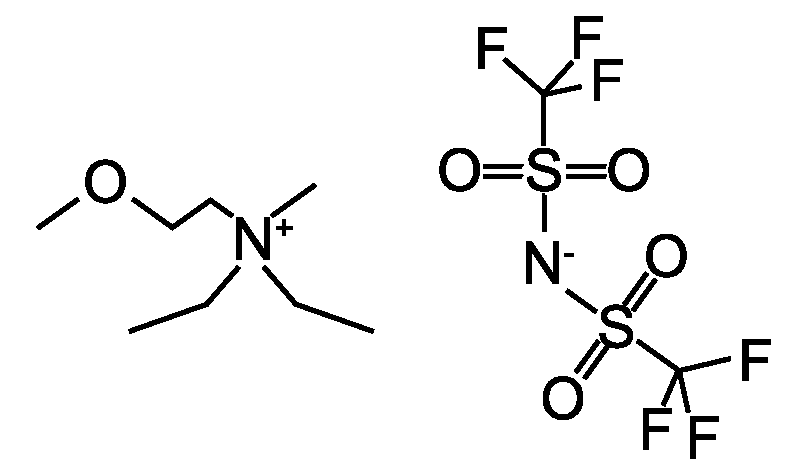
\includegraphics[width=100mm]{images/IL.eps}
\end{center}
 \caption{C$_{8}$H$_{20}$NO.C$_{2}$F$_{6}$NO$_{4}$S$_{2}$の構造式}
 \label{IL}
\end{figure}

かつてはイオン性液体や低融点溶融塩とも呼ばれたこともあるが,"ionic"をイオン性と訳す例が少ないことなどから今ではあまり使われていない.中でも室温において液体で存在できるものを特に室温イオン液体ということもあるが,一般にイオン液体というときは室温イオン液体を指すことが多い.\\


一般的な特徴として,上で述べたように電解質を加えずとも電流が流れ電位窓(有意義な電気化学測定が可能な領域)が広い.また蒸気圧が著しく低くほとんどゼロである.イオン伝導度は$10^{-5}\sim10^{-2}\,\mathrm{Scm^{-1}}$程度が報告されている.さらにイオン液体は耐熱性にも優れる.これらのユニークな性質から様々な分野に応用が期待されている.例えばその一つとして電解質としての利用である.その耐熱性も重なりイオン液体リチウムイオン電池がロケットに搭載されたこともある.その中でスピントロニクスで最もよく用いられる用途は電気二重層(electric doucle layer:EDL)を作成することによるキャリアドーピングである.イオン液体の電位窓の広さから固体ゲートより多くのキャリアドープが可能である点やデバイス作成に関して固体ゲートより簡便に使える点などがメリットとして挙げられる.そこでまずイオン液体による電気二重層の生成について述べたいと思う.その後に本研究で利用したイオン液体によるエッチング作用について述べる.

\subsection{イオン液体による電気二重層}
半導体だけでなくスピントロニクスデバイスにおいてもキャリアの制御はそれらの機能を発展させる重要な鍵になっている.キャリアドープは単なる伝導度を増大させる手段にとどまらず,高いキャリア蓄積は化学反応や相転移,磁気秩序の制御[Y. Yamada, K. Ueno, T. Fukumura, H.T. Yuan, H. Shimotani, Y. Iwasa, L. Gu, S. Tsukimoto, Y. Ikuhara, and M. Kawasaki, Science 332, 1065 (2011).,M. Weisheit, S. Fa ¨hler, A. Marty, Y. Souche, C. Poinsignon, and D. Givord, Science 315, 349 (2007).,K. Shimamura, D. Chiba, S. Ono, S. Fukami, N. Ishiwata, M. Kawaguchi, K. Kobayashi, and T. Ono, Appl. Phys. Lett. 100, 122402 (2012).],さらには超伝導状態の誘起など様々な現象を実現している.\\

長い間半導体であるシリコン(Si)とそれを自然酸化させた酸化シリコン(SiO$_{2}$)薄膜を核にして電界効果トランジスタ(field-effect transistors : FET)を作成するなど電界効果を用いる際は固体酸化物を利用した固体ゲートが主流であった.

しかしながら現在有機化合物やポリマー,複雑な酸化物などの今までの半導体と比較してキャリア数が低い物質がトランジスタの性能向上や今までにない新たな機能の開発において重要な役割を担うと考えられている[21 J. Veres, S. Ogier, G. Lloyd and D. Leeuw, Chem. Mater., 2004, 16, 4543–4555.22 A. Facchetti, M. H. Yoon and T. J. Marks, Adv. Mater., 2005, 17, 1705–1725.23 J. Robertson, Rep. Prog. Phys., 2006, 69, 327–396. ].このような様々な物質に対して十分なキャリアドーピングを行いたいと考えたときにゲート絶縁体が持つべき最も重要な特徴は一定以上のキャパシタンスである.キャパシタンスはゲート電圧を印可したときにどれだけの量のキャリアが誘起されるかを決める.以下ゲート電圧を印可する物質は半導体と考える.平行平板のキャパシタに蓄積した電荷$Q$は
\begin{eqnarray}
Q = CV
\label{eq:capaq}
\end{eqnarray}
と表せる.ただし$C$と$V$はそれぞれキャパシタンスと印可した電圧である.FETにおいてソース-ドレイン間を流れる電流$I_{D}^{SAT}$は飽和領域において
\begin{eqnarray}
I_{D}^{SAT} = \frac{\mu W C}{2L}(V_{G}-V_{G}^{th})^{2}
\label{eq:id}
\end{eqnarray}
と書ける.$L$,$W$はチャンネルの長さ及び幅を表し,$\mu$は移動度,$V_{G}$と$V_{G}^{th})^{2}$はゲート電圧とゲート電圧の閾値を表している.以上の式からわかるのは高いキャパシタンスを持つということは大きい電流が流れることや低いスイッチング電圧だけでなく高いキャリア濃度を誘起することを示している.\\
平行平板のキャパシタンスを思い出すと
\begin{eqnarray}
C = \frac{\epsilon_{0}\epsilon_{r}A}{d}
\label{eq:capa}
\end{eqnarray}
である.($\epsilon_{0}$と$\epsilon_{r}$はそれぞれ真空及び非誘電率,$A$は平行平板の面積,$d$は平板同士の距離である.)イオン液体の$\epsilon_{r}$の値はたかだか$1-10$程度であるがキャパシタンスは$\sim10\,\mathrm{\mu F\,cm^{-2}}$という大きな値を持つ.これはイオン液体が半導体との界面に電気二重層を形成する.電気二重層とは図\ref{EDL}のように半導体のホールとイオン液体のアニオン(陰イオンのこと.正に帯電した陽イオンはカチオンと呼ぶ.)がペアとなった部分のことであり,その結果半導体内にキャリア(ホール)をドープできる.
\begin{figure}[t]
 \begin{center}
  \includegraphics[width=100mm]{images/EDl.png}
\end{center}
 \caption{C$_{8}$H$_{20}$NO.C$_{2}$F$_{6}$NO$_{4}$S$_{2}$の構造式}
 \label{EDL}
\end{figure}

この電気二重層はSiO$_{2}$を用いた固体ゲートによるキャリアドープより何十倍もの効率が実現される[29].例えば例を挙げると厚さ$300\,\mathrm{nm}$のSiO$_{2}$を用いたゲートの持つキャパシタンスは$10\,\mathrm{nF\,\mathrm{cm^{-2}}}$なので,通常の非有機ゲートによる典型的なシートキャリア濃度は$10^{13}\,\mathrm{cm^{-2}}$程度である.この値は半導体の伝導率をある程度制御することは可能であるが,物質をキャリアドーピングによって超伝導状やフェロイック状態に相転移させるようなドラスティックな変化を誘起するには不十分と言わざるを得ない.しかしイオン液体による電気二重層を用いた方法は上記のような現象を発言させることが可能である.なぜならイオン液体によってドープさせるシートキャリア濃度は$10^{15}\,\mathrm{cm^{-2}}$という巨大な値を獲得できるからである.\\
次にイオン液体と固体との界面に形成される電気二重層について述べ,同時にそれのキャパシタンスについても考える.固体と液体との界面についての研究は数多くあり[38-40],それらの界面における電気化学的な振る舞いを説明する様々なモデルが存在する.ここではその中で特に有名な(a)Helmholtzモデル,(b)Gouy– Chapmanモデル(c)Gouy–Chapman–Sternsモデル,そして(d)Multilayerモデルの4つの違いをまとめる.\\


\begin{figure}[t]
 \begin{center}
  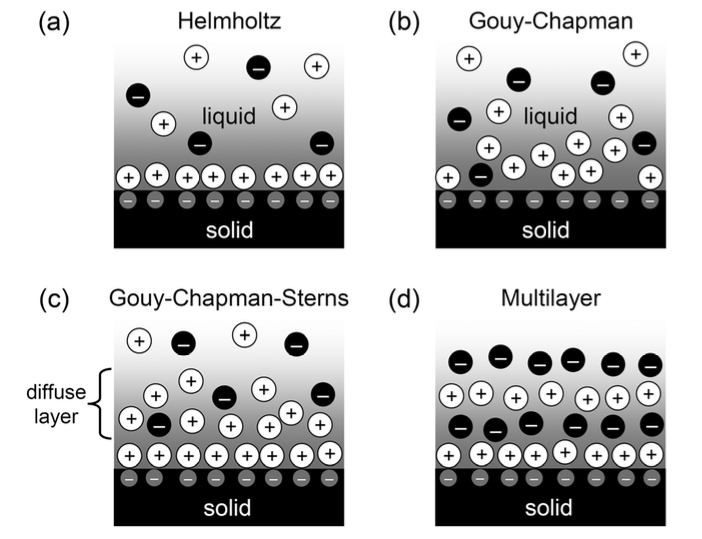
\includegraphics[width=100mm]{images/electrochemicalmodels.png}
\end{center}
 \caption{(a)Helmholtzモデル,(b)Gouy– Chapmanモデル(c)Gouy–Chapman–Sternsモデル,そして(d)Multilayerモデルによる固体/液体界面における電気化学的振る舞い.}
 \label{electrochemicalmodels}
\end{figure}


まず図\ref{electrochemicalmodels}(a)のHelmholtsモデルは液体中のイオンが一層だけ固体表面に層を形成し固体中の電荷を誘起すると考える[41].このモデルの利点は電気二重層のキャパシタンスの計算上の扱いが単純になるということである.そのため用いられるとも多い.一方図\ref{electrochemicalmodels}(b)のGouy– Chapmanモデルは電気二重層自体の拡散を導入している[42,43].\textcolor{blue}{これは固体表面から液体方向にポテンシャルがエクスポネンシャル的に減衰していくことを意味している.}しかしこのモデルだと大きい電気二重層を説明することができない.そこでこの問題を解決するためにGouy–Chapman–Sternsモデルが考案された(図\ref{electrochemicalmodels}(c)).Gouy–Chapman–SternsモデルはHelmholtsモデルとGouy– Chapmanモデルを組み合わせたモデルとなっている.つまり固体表面近傍のイオンが一層を形成しているHelmholtz層とイオンが拡散しているGouy–Chapman層を仮定することにより帯電量の高い電気二重層のキャパシタンスも説明できるようにしている.通常の電解質溶液の溶媒や溶質によるキャパシタンスの振る舞いはこのGouy– Chapmanモデルで十分に説明可能である.しかしながらこれらのモデルは元来希薄した電解質溶液の説明のために考案されたモデルであるため,Debye–Huckel理論[46]のように溶けているイオン同士はよく分離していて互いに相互作用はしないという仮定をおいている.これはイオン液体に関していうと完全に誤った仮定になってしまう.それは室温において溶媒を使わず溶かした"塩"からもよく分かる.そこで考えられたのが図\ref{electrochemicalmodels}(d)のようなMultilayerモデルである.これは融解した"塩"を説明するために確立された.このモデルは界面における空孔がBoltzmann分布に従うと仮定し,これによりイオンの層が多層に渡った構造中の歪みによって分極及びキャパシタンスが説明されている[47,48].このMultilayerモデルは他のモデルと比べて飛躍的によく実験結果を説明できるが,今のところ完全にイオンのみで形成された電解溶液の系を再現するようなモデルは確立されていない.\\

次に実際のイオン液体についての測定例についてまとめる.BaldelliらはBMIM-BF$_{4}$やBMIM-PF$_{6}$,BMIM-DCAなどのイミダゾール化合物(イミダゾール:C$_{3}$H$_{4}$N$_{2}$)をベースとしたイオン液体の表面構造についてマイクロ波(SFG:sum frequency generation)や電気化学インピーダンス(EIS:electrochemical impedance spectroscopy)を用いて研究し[49-52],BMIM-BF$_{4}$とBMIM-PF$_{6}$については隣接した金属との界面におけるイオンがHelmholtz-likeな振る舞いをしていて,そのポテンシャル降下は$3\sim 5\,\mathrm{\AA}$ ほどの範囲で起きていると結論づけている.さらにSFG測定の結果は"二重層"構造がポテンシャルに依存していることを示唆している.つまり\textcolor{blue}{(PZC:potential of zero charge)}が正のときはアニオンは金属表面に吸着しカチオンが持つイミダゾール環は表面に対して垂直に向いている.逆にPZCが負の時はカチオンが表面に対して平行に配向しておりアニオンは表面から離れているということが分かってる.このときの観測されたHelmholtz層の厚さはこの"二重層"を支持した結果になっていたが,アニオンの化学的性質のためBMIM-DCAについてはMultilayerモデルの方がより良く実験結果を再現していた.このときの一層の厚さはおおよそ$25\,\mathrm{\AA}$であった\\
Helmholtzモデルはイオン液体を電極と半導体間に挿入した場合のイオン液体/個体間における電気二重層と電極及び半導体とのポテンシャル差を予測できる.

\begin{figure}[t]
 \begin{center}
  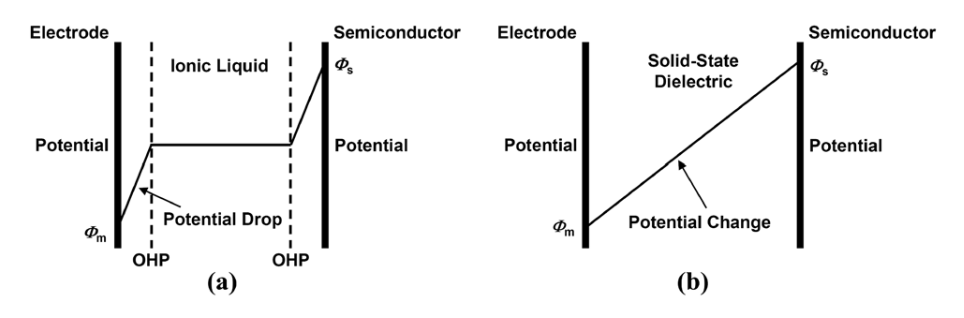
\includegraphics[width=100mm]{images/potentialchanges.png}
\end{center}
 \caption{半導体と電極に挟まれた誘電体((a)イオン液体,(b)固体絶縁体)におけるポテンシャル変化}
 \label{potentialchnages}
\end{figure}

イオン液体では図\ref{potentialchnages}(a)のようにポテンシャル降下はHelmholtz面の外側(OHP:outer Helmholtz plane)に限られる.このポテンシャル降下は電気二重層によるもので極めて薄い範囲で起き,これにより高いキャリア蓄積が半導体に誘起される.またこのOHPまでの距離は電解質の厚さ(イオン液体の種類)にほとんどよらない.この特徴は通常の固体絶縁体を用いたものとは全く異なっている.固体絶縁体中では図\ref{potentialchnages}(b)に示したようにポテンシャル降下は線形なため界面におけるキャリア蓄積は絶縁体の厚さに依存したものになる.


\subsection{イオン液体のキャパシタンス}
ゲート絶縁体のキャパシタンスはそれ自体の性能を判断するときの重要なパラメータである.FujimotoらはEME-TFSIとDEME-BF$_{4}$,BMIM- TFSI,BMIM-BF$_{4}$,BMIM-OTf,BMIM-PF$_{6}$の6つのイオン液体について$10^{-1}\sim10^{5}\,\mathrm{Hz}$の範囲でキャパシタンスの周波数依存性を測定している[53].

\begin{figure}[t]
 \begin{center}
  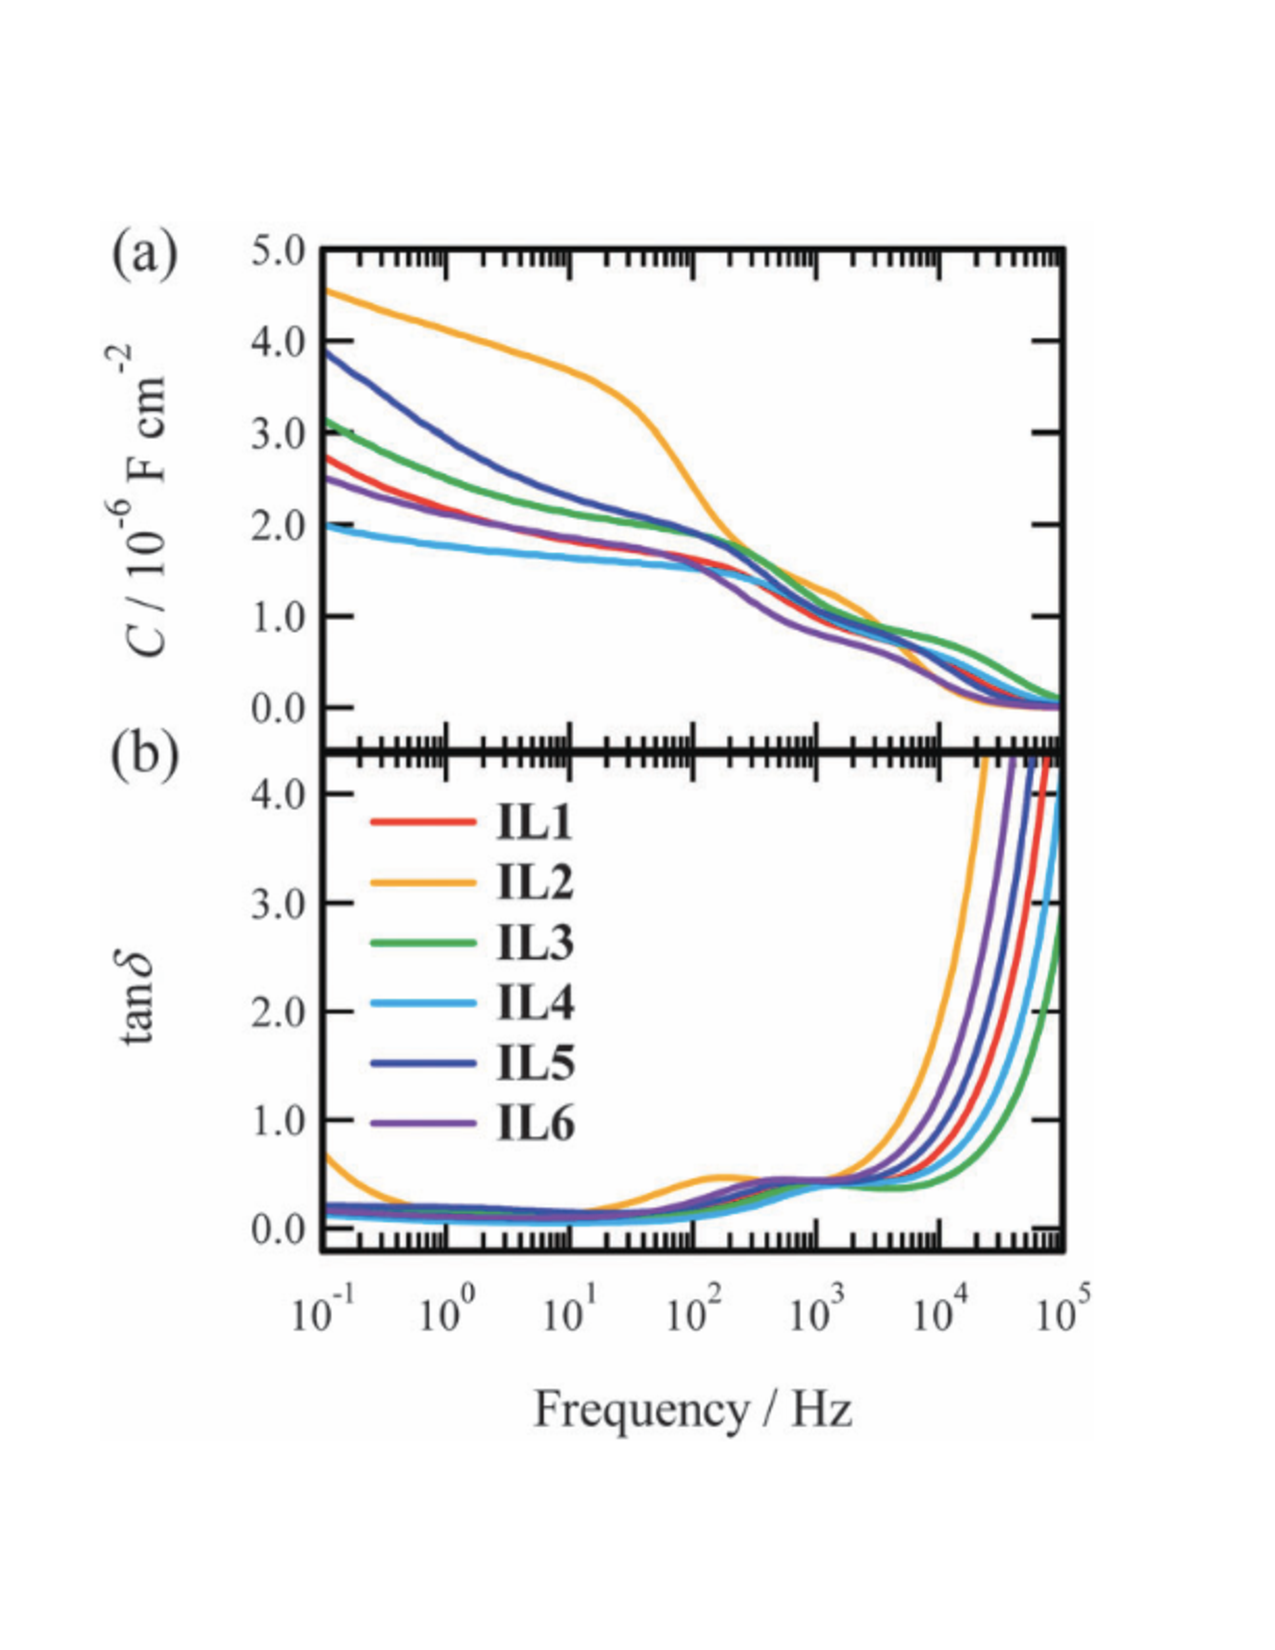
\includegraphics[width=100mm]{images/ILcapacitance.pdf}
\end{center}
 \caption{(a)キャパシタンス及び(b)tan$\delta$の周波数依存性.IL1: DEME-TFSI,IL2:DEME-BF$_{4}$,IL3:BMIM-TFSI,IL4:BMIM-BF$_{4}$,IL5:BMIM-OTf,IL6:BMIM-PF$_{6}$.}
 \label{ILcapacitance}
\end{figure}

その結果が図\ref{ILcapacitance}(a)である.$10^{2}\,\mathrm{Hz}$以下の低い周波数領域ではイオン液体のキャパシタンス$C_{\mathrm{IL}}$の値が$10^{-6}\,\mathrm{F\,cm^{2}}$以上ととても大きく,またイオン液体によって値が大きく異なっている.一方$10^{2}\,\mathrm{Hz}$以上の範囲ではイオン液体の種類によらず同じように減少している.図\ref{ILcapacitance}(b)は損失係数tan$\delta$の周波数依存性を示している.

\begin{figure}[t]
 \begin{center}
  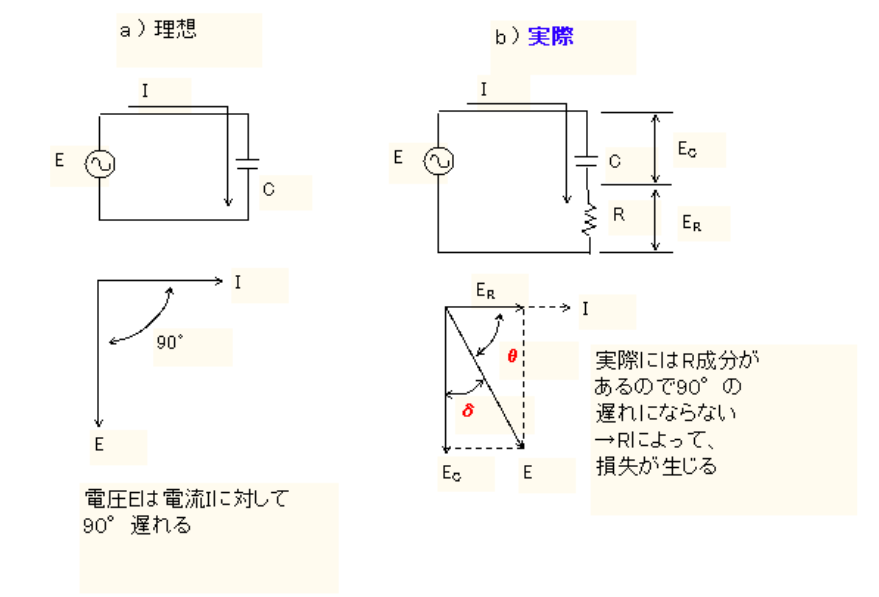
\includegraphics[width=100mm]{images/tandel.png}
\end{center}
 \caption{コンデンサの理想と実際}
 \label{tandel}
\end{figure}

損失係数とはキャパシタンスがどれだけ抵抗成分を含んでいるかを示している値である.図\ref{tandel}のようにキャパシタンス測定において理論的には電圧は電流に対して$90^{\circ}$遅れるはずであるが,実際には回路中の抵抗によってこの位相差が$90^{\circ}$からズレる.このズレの角度を$\delta$とすると損失係数$D$及び品質係数$Q$は

\begin{eqnarray}
\tan\delta = \frac{1}{Q} = D
\label{eq:tandel}
\end{eqnarray}

となる.図\ref{ILcapacitance}(b)を見ると損失係数は$10^{2}\,\mathrm{Hz}$以下で小さく,周波数を増加していくと大きくなっている.また損失係数は以下の式でも表せる.


\begin{eqnarray}
\tan\delta = \frac{I_{\mathrm{R}}}{I_{\mathrm{C}} }= \frac{1}{\omega C_{\mathrm{IL}}R_{\mathrm{P}}}
\label{eq:tandel2}
\end{eqnarray}

ここで$R_{\mathrm{P}}$は並列抵抗及び$\omega$は角運動量周波数であり$I_{\mathrm{R}}$と$I_{\mathrm{C}}$はそれぞれ$C_{\mathrm{IL}}t$と$R_{\mathrm{P}}$に流れる電流である.$R_{\mathrm{P}}$の周波数依存性は線形なので図\ref{ILcapacitance}(b)における$10^{2}\,\mathrm{Hz}$より大きい周波数における損失係数の増大は$C_{\mathrm{IL}}$の低下によるものだと推測できる.このキャパシンタンス及び損失係数の周波数依存性はイオン液体の電気二重層は低い周波数において効果的に現れることを示している.加えてこれらの高い周波数における振る舞いはイオン液体のアニオン及びカチオンが電極界面における空間的に配列しており,その形成が$10^{2}\,\mathrm{Hz}$以上の周波数に対してほとんど追従できていないことを示している.ここからイオン液体は電気二重層が形成がゲート電圧の周波数に追従していると考えられる$10^{2}\,\mathrm{Hz}$以下の周波数において$10^{^6}\,\mathrm{Fcm^{-2}}$という巨大なキャパシタンスを実現し,$10^{15}\,\mathrm{cm^{-2}}$という大きなキャリア蓄積を誘起できるとわかる.これらは通常の固体ゲートと比較して極めて大きな値である.




以上はイオン液体による電気二重層キャパシンタンスを用いることによって固体ゲートに比べ大きな電界効果を与え,効率的かつ簡単にデバイスのキャリア制御を行う方法を述べた.しかし本研究ではこの電解効果を与える作用を用いず,この効果を与えるに有効な電場以上の電場をイオン液体に与えることによって電気分解反応を誘起し接した金属をエッチングする方法のアイデアについて述べたいと思う.

\subsection{イオン液体による電気化学エッチング}


\section{グラフェン}\label{sec:graphene}
グラフェンが物性物理学において注目される物質となり既に10年以上が過ぎている.2005年頃のGeimらのグループ、およひびKimらのグループによるグラフェンの合成及び特異な量子ホール効果の発見[1, 3]によりグラフェンの研究の人気は始まった.現在ではグラフェンの基礎的な研究はほとんどされていると言われているがその応用などの研究を含めれば今でもホットな研究テーマであると言える.この章ではなぜ本研究でグラフェン用いたのかという理由を明白にするため,グラフェンの持つ物理的性質における普遍的な特徴をまとめグラフェンがどれだけ興味深い材料なのかを述べる.そしてスピントロニクスにおけるグラフェンの位置を述べ,これからのグラフェン研究の発展において必要な研究を明らかにし本研究の重要性を述べたい.また本研究で用いたグラフェンは一層のグラフェンであるがグラフェンを数層重ねたグラフェンも同様にグラフェンと呼称する.ここでは誤解を避けるため以下では単層のグラフェンをグラフェンといい,層に言及しない限り単層グラフェン(SLG:single layer graphene)をグラフェンということにする.

\subsection{グラフェンの作成方法}\label{subsec:graphene}
まずグラフェンの作成方法について述べる.グラフェンの作成方法にはいくつか候補がある.代表的なものはFig.\ref{fig:graphene_howtomake}にまとめた.

\begin{figure}[t]
 \begin{center}
  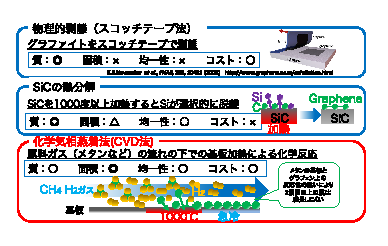
\includegraphics[width=120mm]{images/graphene_howtomake.eps}
  \end{center}
   \caption{グラフェンの代表的な作成方法.}
 \label{fig:graphene_howtomake}
\end{figure}


一つは初めてグラフェンの作成に成功したスコッチテープである.この方法はグラファイトの試料をスコッチテープを用いて剥離を繰り返すことで炭素の層を薄くしていきグラフェンを作成し基板に圧着する.この方法で作成したグラフェンは高品質であることが知られ,最大の移動度を測定されたものもスコッチテープ法で作られた.しかしスコッチテープで剥離を繰り返すため,手に入る試料のサイズは小さく加工も難しい.
SiCの熱分解を用いた方法はその名の通りSiC基盤を1000$\rm\ C^{\circ}$で加熱することにより表面にグラフェンが成長させる方法である.SiCを高温で加熱すると表面においてSiだけが選択的に脱離する.すると表面に残った炭素原子同士が自発的に結合しグラフェンを成長する.この方法によるグラフェンも質が良いことで知られる.しかし大面積のグラフェンを得られてもグラフェンの総数が制御しにくいことやコスト面が高価なためこの方法を選択しなかった.
化学気相蒸着,もしくは化学蒸着(CVD:Chemical Vipor Deposition)法は原料のガス(ここではエタノールガス)を流した中で基板を加熱することで基板表面で化学反応が起きグラフェンが成長する方法である.この方法は他の作成方法に比べグラフェンの質は劣るがコストが低く,基板の選択肢の多さや加工のしやすい.本研究ではこのCVD法を用いてグラフェンを作成した.

\subsection{二次元電子系としてのグラフェン}
この章ではグラフェンの特異な電子状態を述べるために,まずグラフェンの結晶性を物理化学的な構造からまとめる.
グラフェンはFig.\ref{fig:graphene}ベンゼン環が平面状に連なった二次元物質と呼ばれる材料であり,炭素原子がsp$^{2}$混成軌道によりハニカム構造をなしている.
\begin{figure}[t]
 \begin{center}
  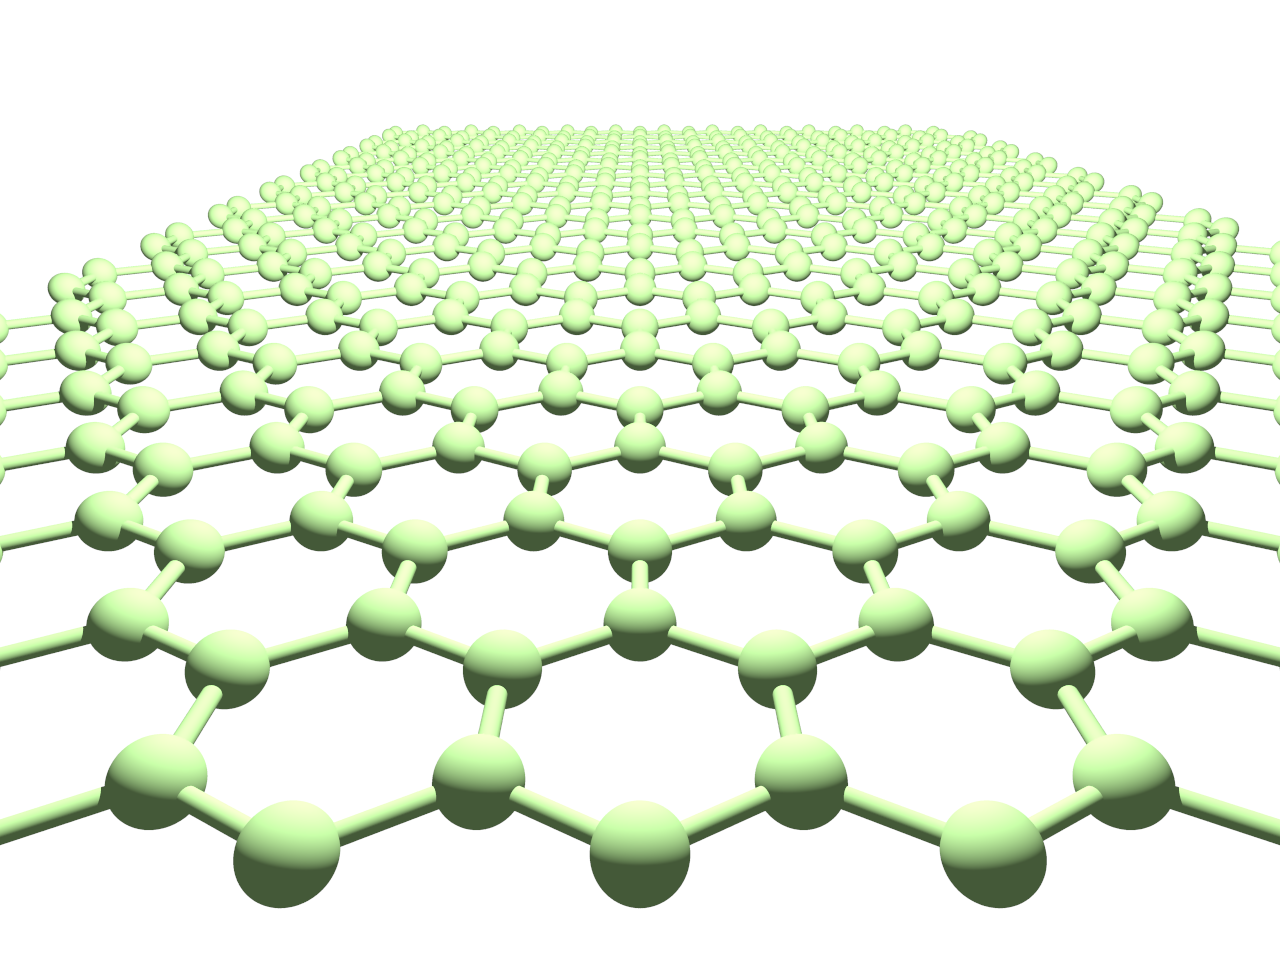
\includegraphics[width=90mm]{images/graphene.png}
  \end{center}
   \caption{グラフェンの概略図.炭素原子がハニカム構造を保って二次元平面状に連なっている.}
 \label{fig:graphene}
\end{figure}

この炭素は強固な共有結合を持つということで有名であり,実際にsp$^{1}$,sp$^{2}$,sp$^{3}$混成軌道という様々な結合状態をもつことを反映し,一次元物質のポリアセチレン,二次元物質のグラフェン,三次元物質のダイアモンドという形態が存在する.(シリコンも炭素と同族であり同じような形態を持つが,自然界に存在するという点では炭素特有である.)
理論的考察からはグラフェンのような二次元物質(しかも十分マクロなサイズで)が合成できるという事実は驚くべきことである.PeierlsやLandau,Merminらが示したように,低次元物質は長波長のエネルギー揺らぎに対して不安定であり,理論的には純粋な一次元や二次元の物質は存在できないと予想されていた[11].しかしこの予想に反してグラフェンは十分大きな面積において二次元構造を維持していると考えられている.このような理論的には存在できない物質が実際に存在できてしまうということが自然科学の面白いと思える部分であり,実験家の存在意義の一つのように感じる.ただしこのストーリーには続きがある.
\begin{figure}[t]
 \begin{center}
  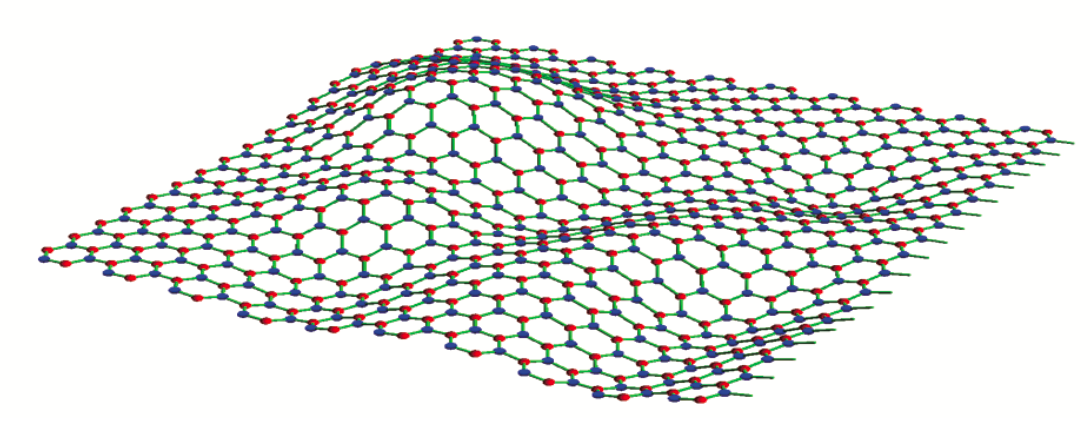
\includegraphics[width=100mm]{images/ripple.png}
  \end{center}
   \caption{グラフェンにおけるリップル構造.これが存在するために二次元構造を保ったまま存在することができると考えられる.}
 \label{fig:ripple}
\end{figure}

実際に存在しているグラフェンを観察すると完全な二次元平面ではなく,Fig.\ref{fig:ripple}のような三次元的な凹凸(リップル:ripple)を持った構造になっており,この長波長のうねりがグラフェンにおいて重要な役割を担っていると考えられている.
つまり二次元物質であっても存在しているのは三次元空間であり自由度も三次元方向に許される.この自由度がゆらぎにおけるエントロピーを吸収し,安定な二次元構造を保っているという考察である.リップルが大きすぎるとsp$^{2}$結合が歪みグラフェン全体の電子系のエネルギー的に損をするため,局所ごとに変形を小さくしそのエネルギー損失を抑えつつ適度なリップルが存在することによりエントロピーを解放するというシナリオのもと,リップルを持った二次元物質が存在できると考えられる.


\subsection{グラフェン中のディラック電子}

次にグラフェンの電子系についてまとめる.
グラフェンの合成は2000年初頭に成功しそこから実際にグラフェンを用いた実験が爆発的に行われたが,理論的には1940年代ごろから考案されておりその特異な電子状態を最初に指摘したのがWallaceである[5].一般的に物質の電子状態は半導体を含む絶縁体と金属に大別される.絶縁体は結晶の周期性による量子力学的干渉効果に起源を持つバンドギャップ構造で特徴付けられ,金属はフェルミ面及びそれをまたぐ電子と正孔の対生成によるギャップレス励起を持つことが知られている.さらに半貴族というカテゴリーがあり,これは通常半導体のギャップレス状態を指す.ギャップレスという意味ではグラフェンも半金属(実際にグラフェンを面直方向に積層したグラファイトは電子及び正孔ポケットを持つ半金属である.)である.しかしグラフェンが特異な点はフェルミエネルギーを貫くバンド分散の傾きがゼロではない(フェルミ速度が有限)点である.これはグラフェンが通常のフェルミエネルギーのバンドの端において電子の速度がゼロになるという常識と反した特異な半金属であるということを示している.この特徴はグラフェンがハニカム構造を持つことに起因する.ハニカム構造はFig.\ref{fig:graphene_vector}のように単位胞中に対称性の異なるに原子を持つ.(図では原子の白と黒で分けている.)

\begin{figure}[t]
 \begin{center}
  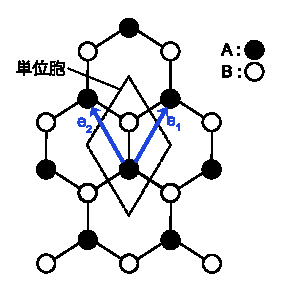
\includegraphics[width=80mm]{images/graphene_vector.eps}
  \end{center}
   \caption{グラフェンのハニカム構造の概要図.点線の範囲が単位胞を表し,対称性の異なる炭素原子サイトを黒円と白円で分けてそれぞれA,Bと表した.$e_{i},i=1,2$は基本並進ベクトルである.}
 \label{fig:graphene_vector}
\end{figure}

この格子はsp$^{2}$混成軌道が互いに$120\ ^{\circ}$異なる三方向に結合していて,化学ではこれを\sigma 結合という.炭素の持つ最外殻電子は4つであり,残りの一つは格子面($x,y$)の垂直方向に伸びたp$_{z}$軌道に入る.この電子が原子間を移動し,この結合を\pi 結合と呼び,この電子によるバンドを\pi バンドと呼ぶ.
実際にグラフェンの電気的性質を担っているのはこの\pi バンドで,フェルミエネルギーもこの\pi バンドを横切っている.これは普通tight-bindingモデルで扱う.このときのハミルトニアンは

\begin{eqnarray}
\mathcal{H} = t\sum_{x}[c_{B}^{\dag}(x)c_{A}(x) + c_{A}^{\dag}(x+e_{1})c_{B}(x) + c_{A}^{\dag}(x+e_{1})c_{B}(x)]
\label{eq:tight-binding}
\end{eqnarray}

のようにかける.ここで$c_{i}^{\dag}$は$i=\rm A$または$\rm B$に電子を生成する生成演算子,$t$は最近接原子への飛び移り積分である.グラフェンにおける実際の値は$t \simeq -3\rm\ eV$である.ハミルトニアンを波数表示するために$c_{i}(x)=\sum_{k}e^{ikx}c_{i}(k)$のようにブロッホ形式に書き直すと

\begin{eqnarray}
\mathcal{H} = \sum_{k}\textbf{\textsl{c}}^{\dag}(k)H(k)\textbf{\textsl{c}}(k),\\
H(k) = 
\begin{pmatrix}
0 & D(k) \\ 
D^{*}(k) & 0  
\end{pmatrix}
\label{eq:tight-binding2}
\end{eqnarray}

となる.ここで$\textbf{\textsl{c}}^{\dag}\equiv(c_{\rm B}^{\dag}(k),c_{\rm A}^{\dag}(k))$,$D(k)=t(1 + e^{\ik_{1}}+e^{\ik_{2}})$である.各$k$ごとに対角化すると永年方程式が$\epsilon^{2}(k)=|D(k)|^{2}$であることからエネルギー分散は$\epsilon(k)=\pm|D(k)|$となることが分かる.またグラフェンのバンド分散はFigのようになり,波数空間の2点($K$点と$K'$点)でエネルギーギャップが線形に交差する.この形をディラックコーンと呼ぶ.この交差してギャップが閉じた点をディラックポイントといい,この点付近の分散関係が質量ゼロのディラック粒子と形式的に類似しているためグラフェン中の電子は相対論的だと表現される.
グラフェンにスピン軌道相互作用があるときディラックコーンのギャップが開く.炭素は軽い原子のためスピン軌道相互作用は弱く,炭素イオンのスピン軌道相互作用による分裂は$7.86\rm\ meV$である.[Kramida, A., Ralchenko, Y., Reader, J. & Team, N. A. NIST Atomic Spectra Database (version 5.1) http://physics.nist.gov/asd (National Institute of Standards and Technology, 2013).]そのため当然グラフェンの内因的なスピン軌道相互作用は小さい.グラフェンのスピン軌道相互作用はバンド状態に強く依存しているため,他原子のドープやゲーティング,基板などの外因的な効果もよく反映する.グラフェンにおけるスピン軌道相互作用の小ささはスピン流の注入や制御の困難さを表すため,グラフェンのスピン軌道相互作用を増大させる方法は注目された研究テーマである.

\subsecton{グラフェンにおける光吸収}
次にグラフェンと光関係についてまとめる.本研究においてグラフェンの評価に用いた測定にラマン分光測定がある.ラマン分光は光の非弾性散乱であり,グラフェンの状態によって光との相互作用が変化するためこれによりグラフェンの評価が可能となる.その基礎としてグラフェンのバンドと光吸収について述べる.

グラフェンは可視光や赤外光などの長波長の光を吸収し赤外光を発光する.このような光吸収と発光に関わっているのがグラフェンにおける\pi バンドである.(価電子帯のバンドを\pi バンド,伝導帯を$\rm\pi^{*}$バンドと呼び分けることもある.)\pi 及び$\rm\pi^{*}$バンドのエネルギーバンドは、ハニカム構造のブリルアン領域の角であるK点,つまりディラックポイントで接する。電子は\pi バンドのみを占有するためフェルミエネルギーはディラックポイントでのエネルギーになる。グラフェンにゲート電圧を加えて電荷を注入した場合には、フェルミエネルギーはこのディラックポイントからずれる。可視光や赤外光などの吸収は\pi バンドから$\rm\pi^{*}$バンドへの遷移によって起こる.可視光より大きなエネルギーを持つ光に対しては、\sigma バンドから$\rm\sigma^{*}$バンドへの遷移や1s軌道から\sigma バンドや$\rm\sigma^{*}$バンドへの遷移によって起こることもある.
光の吸収強度は光の振動する電場ベクトル$E$と原子のもつ遷移双極子モーメントベクトル$D$との内積で与えられる.ここで遷移双極子モーメントとは,光の電場によって原子のまわりの電子分布が変位し負の電荷が誘起され,原子核の正の電荷とともに定義される双極子モーメントのことである・遷移双極子モーメントは光の電場の振動数と同じ振動数で振動するがここで振動の位相が少し遅れる.位相が少し遅れると光が電子に対して仕事をするので光のエネルギーが電子に与えられる.これが光吸収の原理である.光吸収スペクトルの強度は,この遷移双極子モーメントの大きさを入射光のエネルギーの関数として求めることで理論的に計算できる.実験的には光吸収スペクトルを測定することで得られる.上記のようにグラフェンにおける可視光吸収は\pi バンドから$\rm\pi^{*}$バンドへの励起によるが,このときグラフェン1層あたり$2.3 \%$の光が吸収されることが知られている.この吸収強度はグラフェンの層数に比例しているため,光学顕微鏡の元でグラフェンの層数が濃淡で現れる.グラフェン一層の厚さは$0.335\rm\ nm$であるため,グラフェンの光の吸収強度が大きいことがわかる.
光によって励起された電子および価電子帯に発生した正孔がキャリアになり光電流が流れる.光電流とは光を当てた時だけ流れる電流のことを指す.光を当てていない状態で試料に流れる電流を暗電流という.光が当たっていなくても有限温度では電子はフェルミ分布に従って熱的に励起しているので電子とホールを持ち電流を流すことができる.グラフェンでは\pi バンドと$\rm\pi^{*}$バンドは1点で接するのでディラックポイントでの電子の状態密度は0であり電流を担うキャリアの数は少ない.にもかかわらずグラフェンがよく電気を流すのは一つ一つの電荷の移動度の値が非常に大きいからである.電流の大きさは単位体積当たりの電荷の数,一つの電荷の平均速度,電流の流れる断面積の大きさの積で与えられる.一つの電荷の速度は電場と移動度の積で与えられ,移動度は電荷が自由に加速できる時間(緩和時間)に比例し,電荷の質量に反比例する.グラフェンの移動度が大きい理由はディラックポイント付近の電子やホールのエネルギー分散が波数$k$に比例しキャリアーの有効質量がゼロになるからである.有効質量がゼロになるのは相対論的なエネルギーの式$E = \sqrt{m^{2}c^{4} + p^{2}c^{2}}$において$m=0$とおくと$E$が$p=\hbar k$に比例することに対応している.電子のエネルギー$E$が $k$に比例することは非常に特殊な状況である.たとえば電子の群速度は電子のエネルギーによらず一定である.グラフェンの場合には群速度は$106\rm\ m/s$ であり光速の300分の1にもなる.欠陥やフォノンなどで電子が散乱されて運動量の向きが変わっても速度の大きさが変わることはない.フォノンなどの非弾性散乱の場合には,運動量の向きやエネルギーの値は散乱後で変化するが速度は変化しない.特に散乱が無いような結晶性の高い試料でかつフォノンが発生しにくい低温の場合には,移動度は$1\times10^{6}\rm\ cm^{2}/Vs$という驚異的に高い値を示す.したがってTHz領域の高い振動数でも動作可能な素子が作ることができ ることが期待されている.実際にグラフェンで作られたFET(電界効果トランジスター)は$500\rm\ GHz$の遮断周波数(追従できる最高の周波数)が観測されている.

\section{本研究の目的}
本研究の目的はST-FMR測定を用いてDamping-likeトルク及びField-likeトルクを定量する際に単一の試料を用いて膜厚依存性を測定するために,イオン液体の電気化学反応によって強磁性金属をエッチングしながら同時にST-FMR測定を行いトルク定量を実現することである.この研究目的を達成することにより同一試料を作成するのが困難な物質の膜厚依存性や測定とエッチングを同時に行うことが可能になる.つまりこの研究が達成されることによりスピントロニクス分野に限らず材料研究全ての分野の研究進度を加速させることができる.

\section{本論文の構成}
本論文の構成は以下のようになっている.まず第2章で本研究において行った資料作成および実験方法,スピン軌道トルクの定量の仕方について述べる.そして第3章では実際に行った測定について述べ,その結果を説明し考察する.






\chapter{試料作成,ST-FMR測定及びイオン液体を用いた電気化学エッチング方法}
本研究ではNi$_{81}$Fe$_{19}$/Pt二層薄膜構造の試料をST-FMR測定のための電極と共に用意し,その試料におけるNi$_{81}$Fe$_{19}$をイオン液体を用いてエッチングしながらST-FMR測定を行なった.試料のバー及び電極構造はレーザー描画法とリフトオフ法を用いた.金属薄膜の成膜は全てスパッタリング法を用いた.
本章では本研究で用いた試料作成方法とST-FMR測定による電流-スピン軌道トルク生成効率の定量方法,さらにイオン液体を用いた電気化学エッチングの詳細について述べる.

\section{試料設計及び作成方法}
\subsection{スパッタリング法を用いた金属薄膜の成膜}
本研究で用いた金属薄膜試料は全てレーザー描画法により作成した微細構造マスクを用いて成膜した.
試料を成膜した基板はタングステンカーバイドペンにより1.6 cm$\times$1.6 cmの大きさにカットした熱酸化Si基板(Si: 400 $\mu$m,SiO$_2$: 100 $\mu$m)である.金属薄膜を成膜前にSiO$_2$基板をアセトン,エタノールの溶液中に入れ,それぞれ30分間,10分間超音波洗浄を施した.エタノール洗浄後にはN$_2$ガンによりN$_2$ガスを基板上に吹きかけ基板上に残留しているエタノール及び有機物を除去した.
本研究では強磁性金属としてNi$_{81}$Fe$_{19}$,常磁性金属としてPt,電極としてAu/Tiの金属薄膜をそれぞれスパッタリング法により成膜した.ただし,Auに関してはSiO$_2$基板上に単体での均質な薄膜を成膜することが困難であったので(アイランド状に粒を作ってしまう),最初にSiO$_2$基板とAuの接着層としてTiをスパッタリング法により成膜しそのTi上にAuを成膜した.
成膜時の条件を表\ref{tb:deposite condition}に示す.
成膜は最初にArガスの圧力を1 Pa程度に調節した状態で直流(DC)電源で電力を0.1 kWにしてプラズマを発生させた.この状態で高周波(RF)電源を表\ref{tb:deposite condition}のような電力条件にしてつけ,そしてプラズマが安定したところでDC電源をきる.RF電源に切り替えた後に成膜条件のAr気圧となるよう排気の量を調節した.

Ni$_{81}$Fe$_{19}$/Pt二層薄膜及び電極の作成に関して利用したレーザー描画法及びリフトオフ法について次に記述する.

\begin{table}[htbp]
 \caption{金属薄膜成膜時のスパッタリング法の成膜条件.}
 \begin{center}
  \begin{tabular}{cccc}\toprule
  	金属	&	Arガスの気圧	&	電源電力		&	rate (nm/sec)	\\	\hline
	Pt		&	0.23 Pa			&	RF  60 W		&					\\
	Ni$_{81}$Fe$_{19}$ &	0.24 Pa			&	RF  50 W		&	
	\\
	Ti  &   0.24 Pa   &    RF 50 W   &
	\\
	Au  &  0.24 Pa   &   RF 50 W   &   
						\\	\bottomrule
  \end{tabular}
 \end{center}
 \label{tb:deposite condition}
\end{table}

\begin{figure}[htbp]
 \begin{center}
  %\includegraphics[width=85mm]{metalmask.eps}
 \end{center}
 \caption{(a)Ni$_{81}$Fe$_{19}$/Pt二層薄膜構造作成に用いたレーザー描画法における描画パターン,(b)強磁性細線構造作成に用いた電子線描画法における描画パターン及び(c)電極作成に用いたレーザー描画法における描画パターン.
 }
 \label{maskpattern}
\end{figure}





\subsection{レーザー描画法及びリフトオフ法を用いたST-FMR測定系の作成}
レーザー描画法は試料基板に塗布した有機物の膜(レジスト)を感光させ,パターンを作成する方法である.
本研究ではレーザー描画法及びリフトオフ法により目的の試料パターン構造及び電極を作成した.最初にレーザー描画法及びリフトオフ法を用いたバー構造の作成過程について以下に示す.

\begin{figure}[htbp]
 \begin{center}
  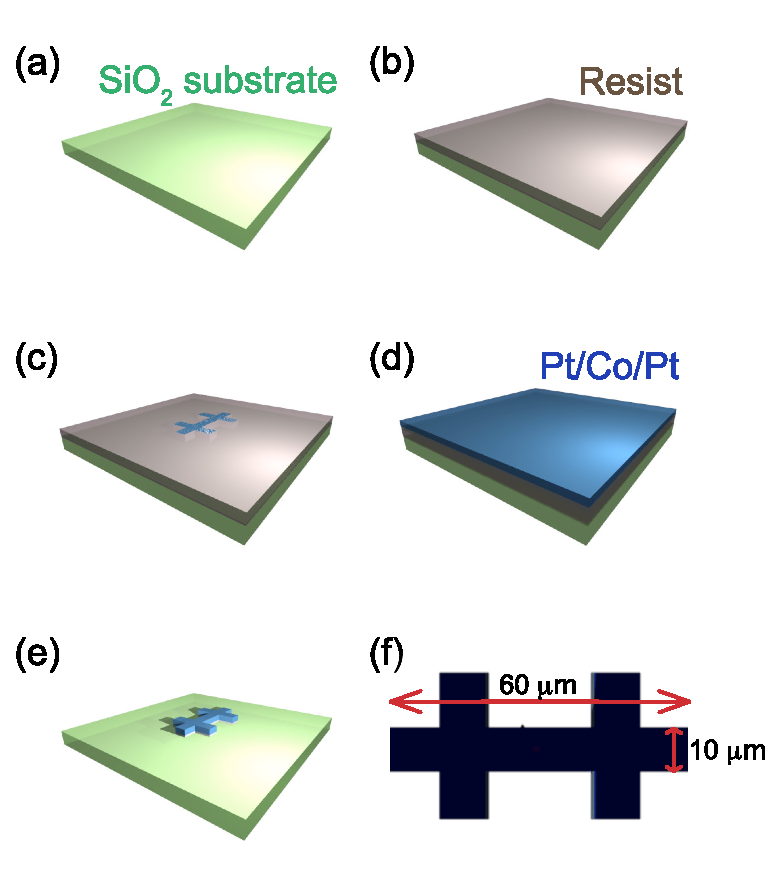
\includegraphics[width=100mm]{images/Making_samples.eps}
 \end{center}
 \caption{(a)-(e)レーザー描画法とリフトオフ法によるNi$_{81}$Fe$_{19}$/Pt二層薄膜構造の作成過程.(a)-(c)に示すようにレーザー描画法を用いてホールバーレジストマスクパターンをSi基板上に作成し、(d)に示すようにNi$_{81}$Fe$_{19}$/Pt層を成膜した後、レジスト層をリフトオフ法によって剥離した(e)。この後同様の流れで電極パターンとしてAu/Tiを成膜した.(f)ホールバーのパターンの大きさを示した.}
 \label{Making_samples}
\end{figure}

熱酸化Si基板をタングステンカーバイトペンを用いて1.6 cm$\times$1.6 cmの大きさにカットした後に超音波洗浄器を用いてアセトンで30分間洗浄し,さらにエタノールにより10分間洗浄してからN$_2$ガンによりエタノールを吹き飛ばし乾燥させた(図\ref{Making_samples}(a)).
次にスピンコーターに洗浄した基板を乗せ,そこにネガ型レジスト溶液(ZPN1150-90)を塗布した.ここで用いたネガ型レジストとは,露光されると感光部分の現像液に対する溶解性が減少し,現像後に露光部分が残るものである.
スピンコーターの条件はまず回転速度500 rpmで5秒間回転させた後,3000 rpmで30秒間回転させた.これにより基板上にレジストを均一に塗布した.その後,$100\rm\ ^{\circ}C$に加熱されたホットプレートで基板を90 秒間ベーキングし,レジスト薄膜を成膜した(図\ref{Making_samples}(b)).
レジスト成膜後はレーザー描画装置を用いてパターン以外の部分に紫外線を照射しパターンをレジスト上に作成した.このときのレーザー描画装置の条件はdefocusが-6でexposure timeが24 msで行った.



レーザー描画した後,基板を$100\rm\ ^{\circ}C$に設定したホットプレートに1分間乗せてポストベークし,現像液(AZ 300MIF DEVELOPER(2.38\%))に42秒浸し,さらにレジストを除去するために純水に1分程度つけることで露光されていない部分を除去した(図\ref{Making_samples}(c)).これによりレジストマスクパターンが完成した.そこへスパッタリング装置を用いて常磁性金属Ptを10 nmを成膜し,その上にさらに強磁性金属Ni$_{81}$Fe$_{19}$を8 nmを成膜した(図\ref{Making_samples}(d)).
成膜後,剥離液であるアセトンに試料をつけ,レジストマスクを剥離した.するとレジストのなかった部分だけが基板上に残り,Ni$_{81}$Fe$_{19}$/Ptのバー上の試料が作成できた(図\ref{Making_samples}(e)).
このようにレジストマスクを作成し,そこへ成膜し,レジストマスクを除去することで所望のパターンを形成する方法をリフトオフ法という.
このホールバーは微小なため,
同様の過程のレーザー描画法により図のような電極パターンのレジストマスクを作成した.
電極はAuを使用したが,金単体ではSi0$_{2}$基板上に安定的に着かず剥がれてしまうのでTiを接着層としてまず成膜しその上にAuを成膜し電極を作成した.その結果が図\ref{madehallbar}である.

\begin{figure}[htbp]
 \begin{center}
  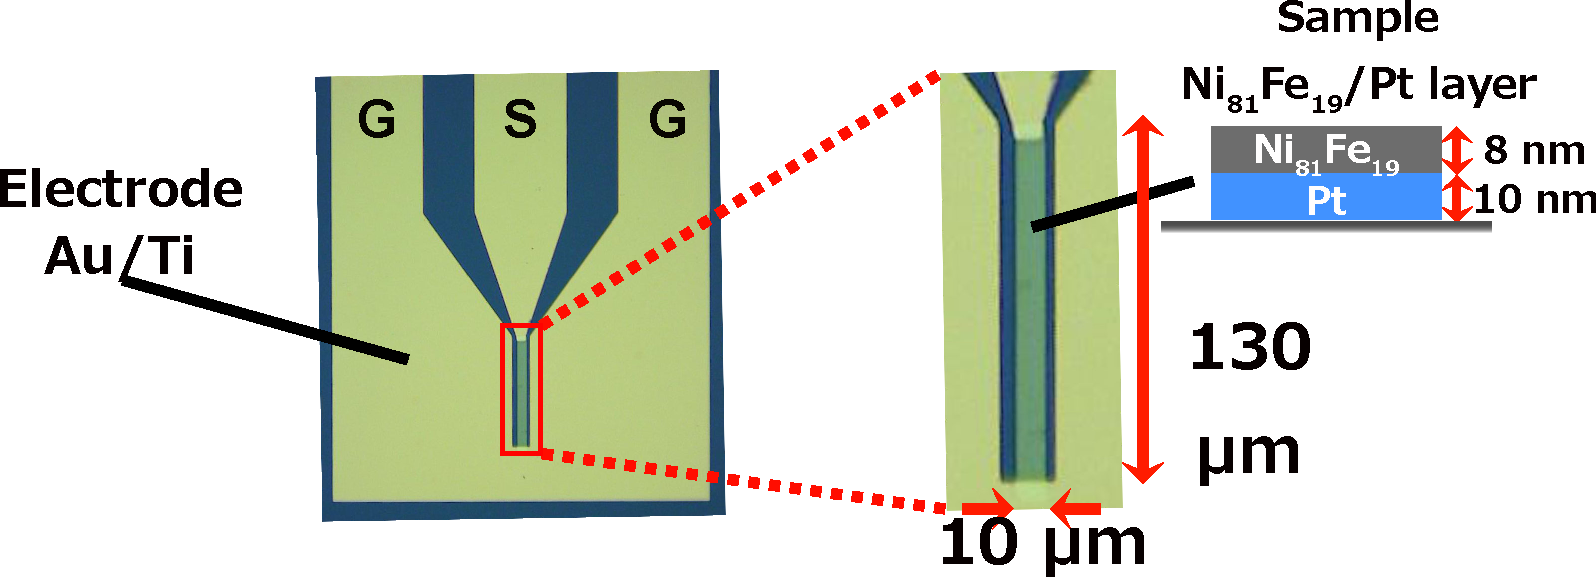
\includegraphics[width=150mm]{images/STFMRpicture.pdf}
 \end{center}
 \caption{作成したホールバーのレーザー顕微鏡図及びレーザー顕微鏡図を拡大した図.右側の細長いバー状の部分がNi$_{81}$Fe$_{19}$/Ptである.}
 \label{madehallbar}
\end{figure}

実際は図\ref{madehallbar}のホールバーおよび電極が1.6 cm$\times$1.6 cmの熱酸化Si基板上に6つ作成できるよう設計図を作成した.
以上のようにしてNi$_{81}$Fe$_{19}$/Pt二層薄膜ホールバー構造及び電極が完成した.


\section{ST-FMR測定を用いた電流-スピン軌道トルク変換効率の定量}\label{FMR_uniform}

この章ではST-FMR測定を用いた電流-スピン軌道トルク生成効率の定量方法について述べる.
ST-FMR測定とは磁化の歳差運動によって強磁性体の抵抗が磁気抵抗効果によって時間依存した変化が起きることを利用した技術である.試料に時間変化する電流$I\cos (\omega t)$を流したとき,その電流によって強磁性体にトルクが与えられその電流と同じ周波数で強磁性体の抵抗が変化する.この電流及び抵抗変化から試料においてDC電圧が生じることになる.この定常電圧$V_{\rm DC}$によって時間の運動を検出することができる.この$V_{\rm DC}$が生じる効果を視覚的に記述するとFig.\ref{fig:frequencymix}のように描ける.

\begin{figure}[htbp]
 \begin{center}
  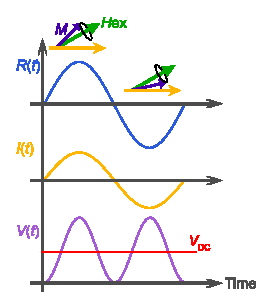
\includegraphics[width=8cm]{images/frequencymix.eps}
 \end{center}
 \caption{$V_{\rm DC}$の生じる原理.歳差する磁化$M$が時間変化する抵抗$R(t)$が生じその周波数はその磁化を歳差させている電流の周波数と同じである.それらの掛け合わせによって電圧$V(t)$が発生し,実際の測定においてはその平均値である定常電圧$V_{\rm DC}$を測定する.}
 \label{fig:frequencymix}
\end{figure}

\subsection{測定系について}

\begin{figure}[htbp]
 \begin{center}
  \includegraphics[width=85mm]{hallbar.eps}
 \end{center}
 \caption{本研究の測定系}
 \label{fig:setup}
\end{figure}
本研究の測定系は図\ref{fig:setup}のようになっている.試料に交流電流$\Delta I\sin\omega t$を流し,電磁石によって外部磁場を試料の面内方向に与える.このときのホール電圧$V_{XY}$は
\begin{eqnarray}
V_{XY} = V_{0}+V_{\omega}\sin\omega t + V_{2\omega}\cos\omega t
\label{eq:Vxy}
\end{eqnarray}
となる.
このホール電圧$V_{XY}$からロックインアンプを用いて高調波Hall電圧$V_{\omega}$と$V_{2\omega}$を測定した.高調波Hall電圧とは流した交流電圧の周波数の整数倍となる周波数で振動するHall電圧のことを指している.

これらの高調波Hall電圧の1次成分$V_{\omega}$と2次成分$V_{2\omega}$からスピン軌道トルクの有効磁場を算出でき,その関係は以下のようになっている\cite{yang2015layer,kim2013layer}.このプレーナーホール効果による電圧が異常ホール効果による電圧に対して微小であるときを想定している.
\begin{eqnarray}
\Delta H_{T(L)}=-2\frac{\partial V_{2\omega}}{\partial H_{T(L)}}\biggl/\frac{\partial^{2} V_{\omega}}{\partial^{2} H_{T(L)}}
\label{eq:torque}
\end{eqnarray}
ただし$H_{T(L)}$は外部磁場を表している.外部磁場を電流に対して平行にかけると$\Delta H_{T}$が測定でき,垂直にかけると$\Delta H_{L}$が測定できる.$\Delta H_{T}$,$\Delta H_{L}$は磁化にかかる有効磁場で添え字のTやLは電流に対して平行か垂直かを表している.

試料が面直磁化容易膜(面直磁化膜)である場合,有効磁場$\Delta H_{T}$はfield-likeトルクを,$\Delta H_{L}$はdamping-likeトルクを起源としているとわかっている\cite{yang2015layer}.そこで,本研究ではこの有効磁場$\Delta H_{T(L)}$の変化をスピン軌道トルクの変化として扱うことにする.

\subsection{スピン軌道トルクの導出}


%以上の計算はプレーナーホール効果による電圧を無視して考えているため電流と磁場の方向によって$\Delta H_{T(L)}$を分離することができている.プレーナーホール電圧による寄与を無視するということは電流に対して平行な磁化の動きに対応する電圧を無視するということを意味する.実際の磁化の動きは図\ref{harmonicFig}のように表せる.垂直磁化膜の磁化は図\ref{harmonicFig}(a)のような平衡状態にある.そこに交流電流を流し外部磁場を印加すると図\ref{harmonicFig}(b)(c)のように磁化が動く.


%図(\ref{harmonicFig})において(b)では$\Delta H_{T}$によって,(c)では$\Delta H_{L}$によってプレーナーホール電圧が誘起されるはずである.









\subsection{イオン液体を利用した電気化学エッチングの方法}

イオン液体

%本研究では磁化ダイナミクス励起及び磁化ダイナミクスの解析に電子スピン共鳴(Electron Spin Resonance: ESR)装置を用いた。電子スピン共鳴装置は測定試料に固定角周波数$\omega$のマイクロ波を照射し、外部直流磁場$H$を掃印した際の
%試料によるマイクロ波吸収を測定するものである。以下では電子スピン共鳴装置により得られる強磁性共鳴スペクトルと磁化ダイナミクスの関係を示す。

%強磁性体中の磁化ダイナミクスは式(\ref{LLG})のLLG方程式に従う。式(\ref{LLG})は磁化が有効磁場$\bm{H}_\text{eff}$を軸として歳差運動を行い、スピン角運動量やエネルギーを散逸して$\bm{H}_\text{eff}$方向に緩和することを示している。
%磁化歳差運動の角周波数と等しい角周波数を持つマイクロ波を照射すると、磁化はマイクロ波からエネルギーを吸収して減衰することなく歳差運動を続ける。これが強磁性共鳴である~\cite{Chikazumi}。


%強磁性共鳴によるマイクロ波の吸収スペクトルから、磁化ダイナミクスを支配するパラメータの一つである緩和定数$\alpha$を実験的に求めることが可能である\footnote{$\alpha$は歳差運動の緩和時間$\tau$を定めるパラメータである。
%LLG方程において有効磁場$\bm{H}_\text{eff}$が$z$方向を向いている場合を考える。
%歳差運動の振動成分$m_x$, $m_y$の解を$(m_x,\; m_y)=m_0 e^{-t/\tau}(\cos\omega t,\; \sin\omega t)$とする。
%$\tau$は歳差運動の緩和時間である。$M_s^2=m_x^2+m_y^2+M_z^2$から$M_z=M_s\left(1-(m_0/M_s)^2 e^{-(2t/\tau)}\right)^{1/2}$となり、時間経過によって$M_z=M_s$に緩和する。また$m_x$, $m_y$をLLG方程式に代入すると
%$d M_z/dt=(\alpha/M_s)m_0^2\omega e^{-2t/\tau}$
%が得られる。この2式より$
%\alpha\tau\omega=\left(1-(m_0/M_s)^2e^{-2/\tau}\right)^{-1}$
%となり、微小振動$(m_0/M_s)^2\ll 1$の範囲では緩和時間$\tau$と緩和定数$\alpha$の間に
%\begin{equation}
%\tau\simeq 1/\alpha\omega\nonumber
%\end{equation}
%の関係がある。
%}。
%この概要を以下に示す。
%外部直流磁場$H$とマイクロ波磁場$h$を考え$\bm{H}=(h\cos \omega t,h\sin \omega t,H)$とする。複素磁化率$\chi=\chi'-i\chi''$を導入すると、同位相応答の磁化$M'$と$\pi /2$位相遅れの磁化$M''$の$y$成分は
%$M_y'=\chi 'h\sin \omega t$及び$M_y''=-\chi ''h\cos \omega t=\chi ''h\sin (\omega t-\pi /2)
%$となる。強磁性試料によるマイクロ波吸収は単位時間あたりの磁気的エネルギーの変化分$H(dM/dt)=Hd(M'+M'')/dt$に対応するため、強磁性共鳴によるマイクロ波吸収量$I$は
%振動磁場一周期あたりのマイクロ波吸収の時間は$2\pi /\omega$であるので、全吸収量は
%\begin{eqnarray}
%I=\frac{\omega}{2\pi}\int^{2\pi/\omega}_0 \bm{H}\cdot\frac{d\bm{M}}{dt}dt
%=\frac{1}{2}\omega\chi'' h^2\label{absorption}
%\end{eqnarray}
%となり、複素磁化率の虚数成分$\chi''$に比例する。

%磁化率の虚数成分は強磁性薄膜面内に磁場を印加した場合
%\begin{equation}
%\chi '' = \frac{\alpha{M_s}\left( H_\text{FMR} + 4\pi {M_s} \right)  }{2\left( H_\text{FMR} + 2\pi {M_s}  \right)}\frac{\left(\omega/\gamma\right)}{ (H - {H_\text{FMR}})^2+\left(\alpha\omega/\gamma\right)^2}
%\end{equation}
%で与えられる\footnote{第\ref{formulation}章 式(\ref{chi3})参照}。ここで$H_\text{FMR}$は強磁性共鳴磁場を表す。従って式(\ref{absorption})より、共鳴磁場付近($H\approx H_\text{FMR}$)におけるマイクロ波吸収量$I$はローレンツ関数
%\begin{equation}
%I(H) = \frac{1}{4 } {M_s}  h^2\gamma\left(\frac{{ {{H_\text{FMR}} + 4\pi {M_s}}  }}{  H _\text{FMR}+ 2\pi {M_s} }\right)\frac{\alpha  (\omega/\gamma)^2}{ { {{(H - {H_\text{FMR}})}^2}+(\alpha \omega /\gamma)^2 } }\label{absorption2}
%\end{equation}
%となる。
%電子スピン共鳴装置では磁場変調によるロックイン法を用いているため、測定される吸収スペクトルは図\ref{FMR}に示すような式(\ref{absorption2})の微分形$dI(H)/dH$である。
%図\ref{FMR}に定義した微分吸収曲線のピーク間線幅$W$は式(\ref{absorption2})より
%\begin{equation}
%W=\frac{2\omega}{\sqrt{3}\gamma}\alpha \label{Wtoa}
%\end{equation}
%で与えられる。従って電子スピン共鳴装置を用いた強磁性共鳴によるマイクロ波吸収スペクトルのスペクトル線幅$W$からスピン緩和定数$\alpha$を得ることができる。
%一方ピーク間強度$S$は式(\ref{absorption2})より
%\begin{equation}
%S=\frac{3\sqrt{3}M_s \gamma^2 h^2 (H_\text{FMR}+4\pi M_s )}{16  (H_\text{FMR}+2\pi M_s)\omega\alpha^2}\label{strength}
%\end{equation}
%であり、$1/\alpha^2$に比例する。


%\begin{figure}[tbp]
% \begin{center}
  %\includegraphics[width=40mm]{FMR.eps}
% \end{center}
% \caption{マイクロ波吸収スペクトル$dI(H)/dH$。$I$はマイクロ波吸収強度、$H$は外部磁場である。スペクトル線幅$W$及びスペクトル強度$S$の定義を示した。
%}
% \label{FMR}
%\end{figure}


%
\chapter{PdO$_{\rm x}$の電流-スピン軌道トルク変換効率に関する研究}

\section{PdO$_{\rm x}$/Ni$_{81}$Fe$_{19}$薄膜の作成}

\section{PdO$_{\rm x}$/Ni$_{81}$Fe$_{19}$薄膜のST-FMR測定および電流-スピン軌道トルク変換効率の定量}

\chapter{イオン液体を用いた電気化学エッチングによるST-FMR測定の強磁性体膜厚依存性}\label{ILEtchingchap}
本章ではイオン液体の電気化学効果を利用したエッチングに関する測定とその結果を述べ考察する.本研究は強磁性体/常磁性体二層薄膜構造におけるスピン軌道トルクの生成効率を定量する際に必要な強磁性体膜厚依存性をイオン液体の電気化学エッチングを用いて測定することを目指したものである.この測定が可能になることで複数の試料が作成困難な試料のトルク定量が可能になるだけでなく,強磁性体のばらつきが測定に含まれないためより精密な測定結果を得られることが見込まれる.本研究ではもっとも簡単で多くのグループで研究がされているNi$_{81}$Fe$_{19}$/Pt系を用いて上で述べた測定系の確立に臨む.


%SAMのない試料はCoに対するPtの対称性により,Co内の磁化にトルクがほとんどかかっていないと考えられる.その表面にSAMを形成したことでSAMによるスピン軌道トルクのみがCoの磁化に与えられその影響を定量できる.


%\part{逆スピンホール効果の面外磁場角度依存性}\markright{第\thepart 章 逆スピンホール効果の面外磁場角度依存性}
%強磁性/常磁性金属複合系における逆スピンホール効果を用いたスピン流の電気的検出を実現し、磁化ダイナミクスによるスピン流生成及び逆スピンホール効果によるスピン流−電圧変換を系統的に調べた。
%スピン流と磁化ダイナミクスが結合する
%スピンポンピングによるスピン流生成及び逆スピンホール効果によるスピン流−電流変換を実現する
%最も簡単な系であるNi$_{81}$Fe$_{19}$/Pt複合薄膜において、
%強磁性共鳴により駆動されるスピンポンピングはPt層へスピン流を注入する。このスピン流は逆スピンホール効果によって起電力へと変換される。強磁性共鳴測定と同時にPt層両端に生じる起電力測定を行い、マイクロ波の共鳴吸収に起因するローレンツ関数型の起電力信号を検出した。この起電力信号のマイクロ波強度依存性及び外部磁場角度依存性を体系的に調べ、現象論的な直流スピンポンピングによる逆スピンホール効果の模型と整合する結果を得た。

%\section{SAMの形成についての確認}

%\subsection{光電子分光測定}

\section{Ni$_{81}$Fe$_{19}$/Pt二層薄膜のST-FMR測定及びNi$_{81}$Fe$_{19}$膜厚依存性の測定}

この章ではまずイオン液体を用いずNi$_{81}$Fe$_{19}$/Pt二層薄膜のST-FMR測定及びNi$_{81}$Fe$_{19}$膜厚依存性を測定し,本研究室において以上のトルク定量が他のグループの結果を再現するかを確認した結果を述べる.

\subsection{Ni$_{81}$Fe$_{19}$/Pt二層薄膜のST-FMR測定}
まずNi$_{81}$Fe$_{19}$/Pt二層薄膜のST-FMR測定結果について述べる.

ST-FMR測定の周波数依存性を測定した結果がFig.\ref{fig:initial_FMR}である.このとき用いたマイクロ波電流のパワーは$100\rm\ mW$である.それぞれのスペクトルの色がマクロは電流の周波数を表しており,$4\rm\ GHz$から$10\rm\ GHz$まで$0.5\rm\ GHz$ごとに測定した.スペクトルの強度が変化しているのは電極の周波数特性を反映しているがトルク生成効率の定量には基本的に影響はない.

\begin{figure}[htbp]
\centerline{
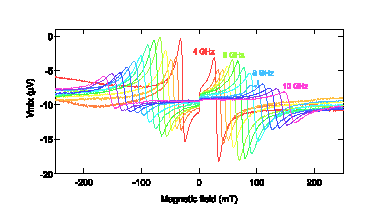
\includegraphics[width=10cm]{images/initial_FMR.eps}
}
\caption{Ni$_{81}$Fe$_{19}$/Pt二層薄膜のST-FMRスペクトル.$4\rm\ GHz$から$10\rm\ GHz$まで$0.5\rm\ GHz$ごとに測定したもの.
}
\label{fig:initial_FMR} 
\end{figure}

この測定したそれぞれのFMRスペクトルをフィッティングすると対称成分$V_{\rm sym}$と反対称成分$V_{\rm asym}$に分離することができる.例えば$7\rm\ GHz$のスペクトルの$V_{\rm sym}$と$V_{\rm asym}$を分離してまとめた結果がFig.\ref{fig:Vseparate}である.\textcolor{blue}{前の章で述べたように}対称成分$V_{\rm sym}$にはdamping-likeトルク,反対称成分$V_{\rm asym}$にはfield-likeトルクの寄与が強く含まれている.この分離をするために強磁性体膜厚依存性が必要である.

Fig.\ref{fig:initial_FMR}の周波数依存性及びフィッティング結果からわかることも多い.

まず共鳴周波数と共鳴磁場の関係からKittelの公式を用いるとNi$_{81}$Fe$_{19}$の飽和磁化が定量できる.その結果がFig.\ref{fig:kittel_initial}である.これらの結果から飽和磁化は$644.29 \pm 0.78\rm\ mT$(正磁場側),$661.56 \pm 1.9\rm\ mT$(負磁場側)と定量できた.



\begin{figure}[htbp]
\centerline{
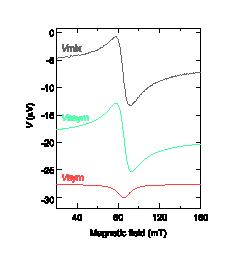
\includegraphics[width=8cm]{images/Vseparate.eps}
}
\caption{Ni$_{81}$Fe$_{19}$/Pt二層薄膜のST-FMRスペクトルに含まれる対称成分$V_{\rm sym}$と反対称成分$V_{\rm asym}$(ただし$7\rm\ GHz$で測定したもの).
}
\label{fig:Vseparate} 
\end{figure}


\begin{figure}[htbp]
\centerline{
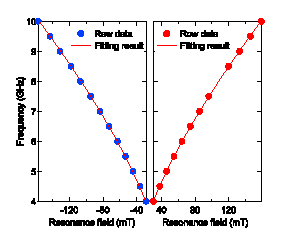
\includegraphics[width=8cm]{images/kittel_initial.eps}
}
\caption{共鳴周波数と共鳴磁場の関係.この関係はKittelの式で表すことができる.青のデータが負磁場,赤のデータが正磁場側の結果である.フィッティング結果はKittelの式の飽和磁化をフィッティングパラメータとしている.
}
\label{fig:kittel_initial} 
\end{figure}

また前に述べたようにスペクトル線幅$W$の周波数依存性から試料のダンピング定数$\alpha$及び不均一線幅が定量できる.スペクトル線幅$W$にはスピン流などのスピン角運動量のダイナミクスによる線幅の変化と強磁性体の不均一性から生じる線幅の変化が含まれる.それらを分離するために周波数依存性を測定した.線幅の周波数依存性の結果はFig.\ref{fig:V-f}に示した.この結果からダンピング及び不均一幅が定量できる.不均一線幅は$0.050\rm\ mT$だった.ここあらこの実験で用いたNi$_{81}$Fe$_{19}$の不均一性は小さいと言える.
\begin{figure}[htbp]
\centerline{
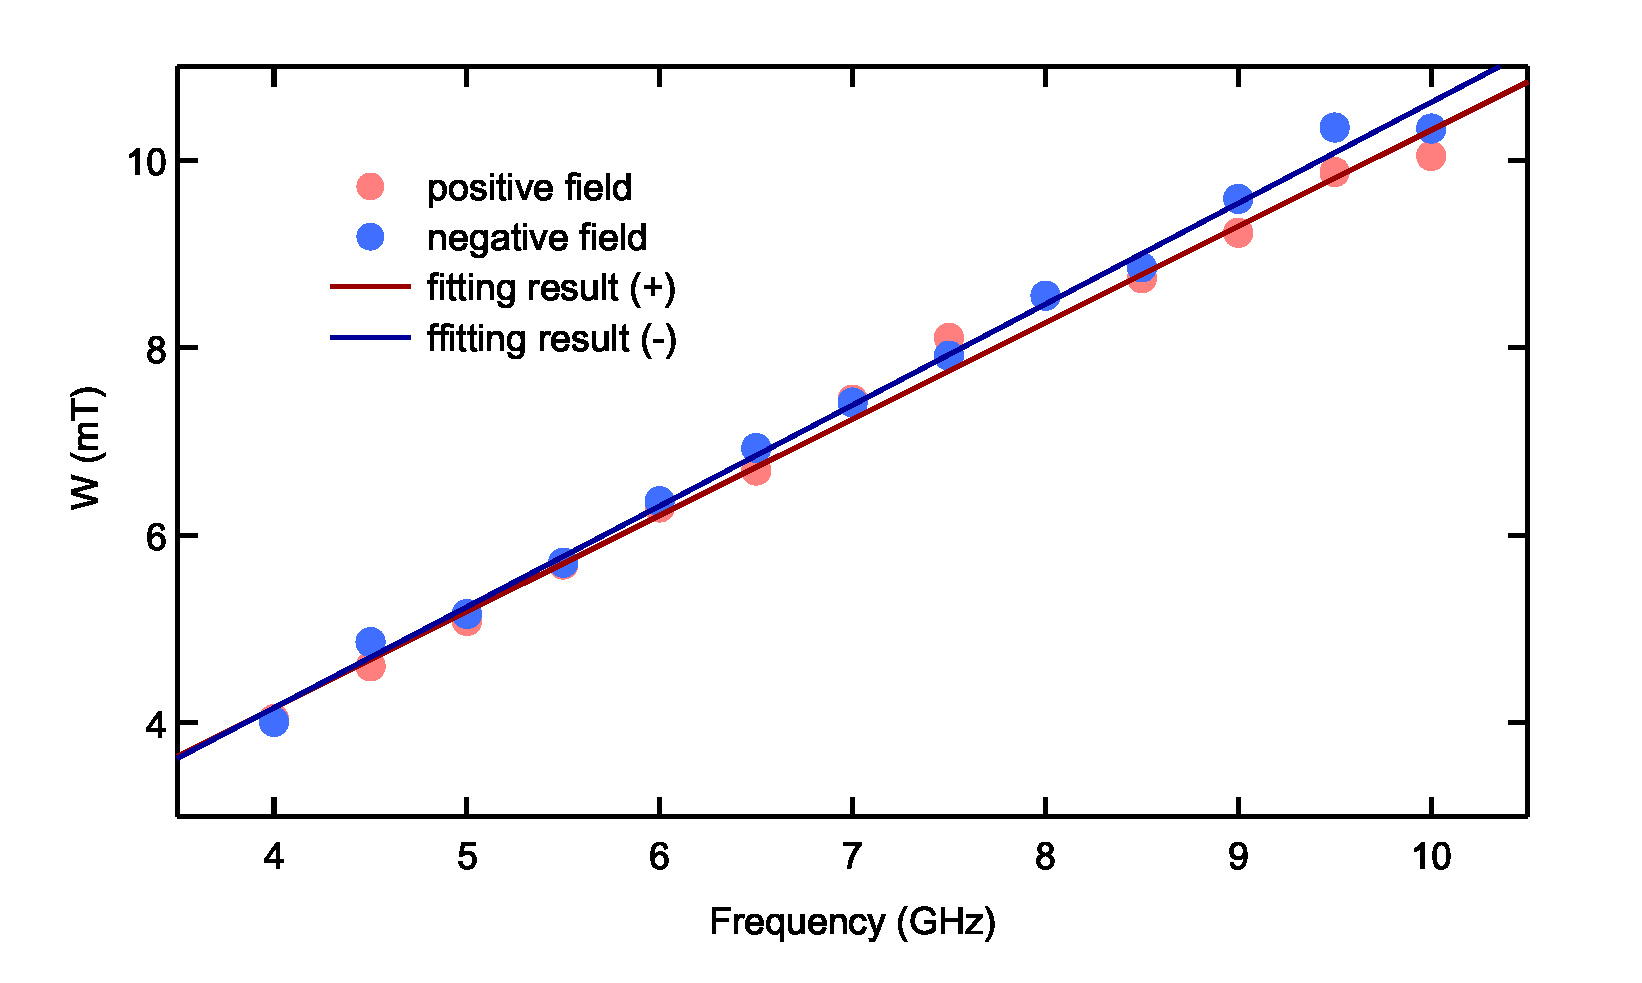
\includegraphics[width=10cm]{images/W-f.eps}
}
\caption{Ni$_{81}$Fe$_{19}$/Pt二層薄膜のスペクトル線幅の周波数依存性.青のデータが負磁場側のスペクトル,赤のデータが正磁場側のスペクトルの結果である.
}
\label{fig:V-f} 
\end{figure}


次にFig.\ref{fig:initial_FMR}の結果から電流-スピン軌道トルク生成効率$\xi_{\rm FMR}$を求めた結果を述べる.スペクトルから$V_{\rm sym}$と$V_{\rm asym}$の比をを求め,Fig.\ref{fig:W-f.eps}から求めた飽和磁化を用いて算出する.まず正磁場及び負磁場のスペクトルから求めた$\xi_{\rm FMR}$はFig.\ref{fig:xi_initial}に示した.ここからPtの$\xi_{\rm FMR}$は0.06程度だと見積れる.この結果は他のグループの報告と一致しており,Ptの$\xi_{\rm FMR}$を再現できていると考えられる.この結果からdamping-likeトルク及びfield-likeトルクの生成効率を見積もるため,Ni$_{81}$Fe$_{19}$の膜厚依存性を測定した.この結果と比較することでイオン液体によるエッチングから求めた結果が妥当なものであるかを検討する.

\begin{figure}[htbp]
\centerline{
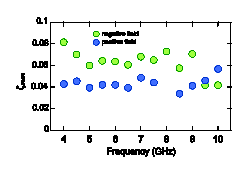
\includegraphics[width=10cm]{images/xi_initial.eps}
}
\caption{Ni$_{81}$Fe$_{19}$/Pt二層薄膜における電流-スピン軌道トルク生成効率$\xi_{\rm FMR}$の周波数依存性.緑の円が負磁場側,青の円が正磁場側のスペクトルから定量した結果.
}
\label{fig:xi_initial} 
\end{figure}




\section{イオン液体によるNi$_{81}$Fe$_{19}$薄膜のエッチング}
\label{sec:PyPt}
この章ではまずイオン液体によってNi$_{81}$Fe$_{19}$をエッチングする方法の模索について述べる.本研究の最初はゲート電圧の印可方向を正方向に設定しエッチングをしていたが,負方向にすることでスムーズなエッチング及びST-FMR測定結果を得られることを発見した.その過程を以下にまとめる.

\subsection{イオン液体による電気化学エッチング -正のゲート電圧-}
本研究は塩貝らが超伝導体をイオン液体の電気化学効果によってエッチングした方法\textcolor{blue}{[]}に着目して始まった.そのためまず塩貝らと同様の方法でイオン液体にゲート電圧を印可した.というのも塩貝らの論文にはFig.\ref{fig:shiogai}のような模式図がありこのゲート電圧の印可方向は一般的なゲート電圧と同方向であるため,本研究でも最初はこのゲート電圧方向を採用した.

\begin{figure}[htbp]
\centerline{
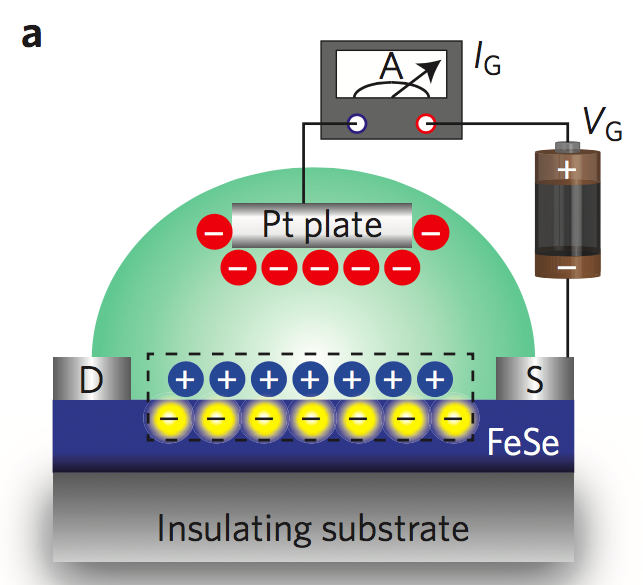
\includegraphics[width=7cm]{images/shiogaireport.png}
}
\caption{塩貝らのイオン液体による超伝導体(FeSe)のエッチング方法の模式図\textcolor{blue}{[]}.エッチングする超伝導体側がゲート電圧の負側になっている.
}
\label{fig:shiogai} 
\end{figure}

本研究ではまずイオン液体によってNi$_{81}$Fe$_{19}$薄膜がエッチングされるのかを確認するために,エッチングのためのゲート電圧を印可しその時の試料の抵抗変化を測定した.このときの測定系はFig.\ref{fig:IL_resi_setup}に示したような回路で表せる.エッチングの可否を点A-B間の抵抗$R_{\rm AB}$の変化によって確認した.ただしこの$R_{\rm AB}$には試料(Ni$_{81}$Fe$_{19}$(8)/Pt(10))の抵抗に加え接触抵抗及び金電極の抵抗が含まれている.

\begin{figure}[htbp]
\centerline{
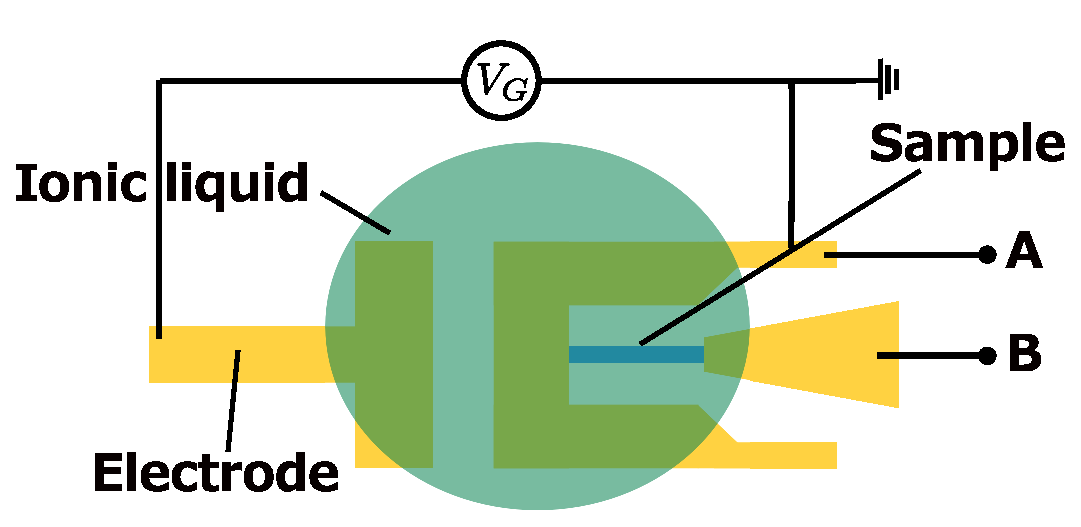
\includegraphics[width=7cm]{images/IL_resi_setup.eps}
}
\caption{ST-FMR測定系での抵抗測定の模式図.点A-B間の抵抗$R_{\rm AB}$を測定しエッチングによるその変化を追跡した.
}
\label{fig:IL_resi_setup} 
\end{figure}



\begin{figure}[htbp]
\centerline{
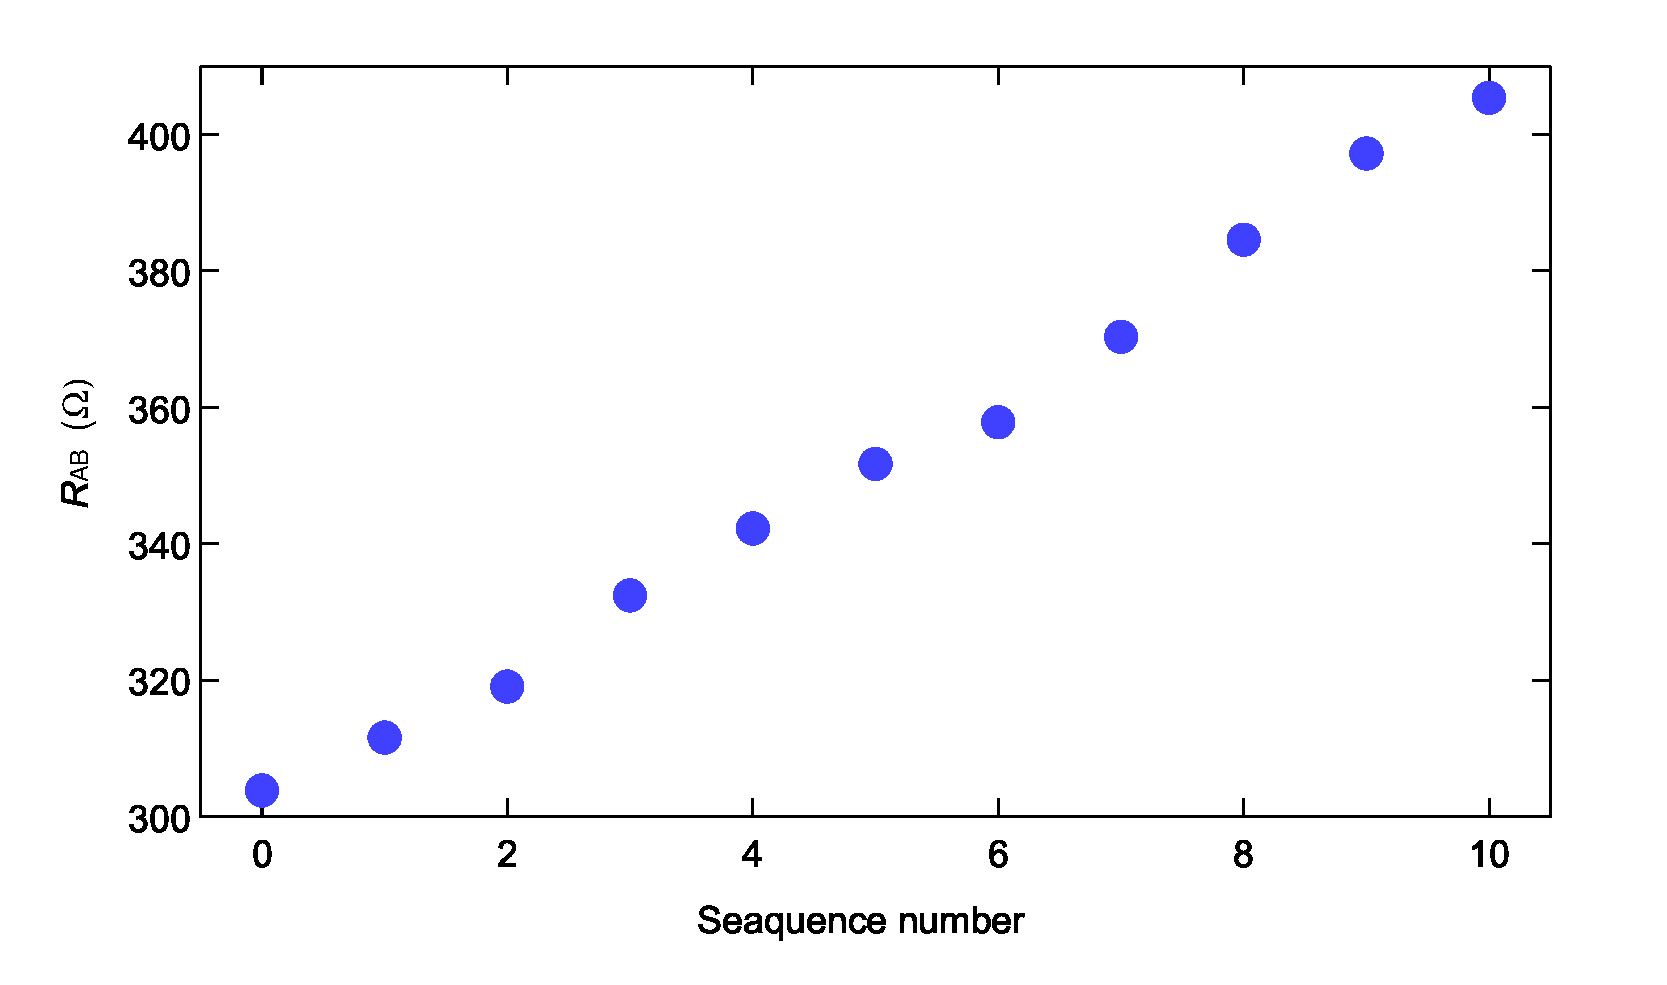
\includegraphics[width=7.5cm]{images/resichange_before.eps}
}
\caption{イオン液体によるエッチングによる$R_{\rm AB}$の変化.イオン液体にゲート電圧5Vを15 sec印可しその後60 sec待機するという操作を一つのシークエンスとしてそれを9回繰り返した結果である.
}
\label{fig:resichange_before} 
\end{figure}

実際にエッチングしながら抵抗測定した結果がFig.\ref{fig:resichange_before}である.x軸のシークエンスというのは,ゲート電圧5 Vを15 sec印可しその後60 sec待機するという流れをエッチングプロセスの一つのシークエンスとしたときの何度エッチングしたかという値である.このときゲート電圧を5 V以下にするとこのような大きな抵抗変化は見られなかった.実際に何時間もの間電圧を印可し続ければエッチングできる可能性もあるが,ある電圧以上でエッチングされる閾値が存在すると推測でき,この結果は他のグループの報告にも一致する.Fig.\ref{fig:resichange_before}を見ると最初の抵抗の値が$303.08\rm \Omega$だったのがエッチングを繰り返すことで$405.5\rm \Omega$と抵抗が増加していることがわかる.ここからイオン液体を用いて実際にNi$_{81}$Fe$_{19}$薄膜の膜厚が減少,つまりエッチングされ得ることが分かった.

そこでこのエッチングを用いてNi$_{81}$Fe$_{19}$/Pt二層薄膜のST-FMR測定を行い,Ni$_{81}$Fe$_{19}$の膜厚依存性を測定した.その結果がFig.\ref{fig:meltingFMR_before}である.

\begin{figure}[htbp]
\centerline{
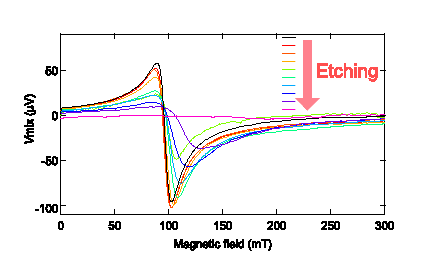
\includegraphics[width=9cm]{images/meltingFMR_before.eps}
}
\caption{イオン液体によるエッチングを利用したFMRの膜厚依存性.黒の線が初期状態を表している.
}
\label{fig:meltingFMR_before} 
\end{figure}

この図を見るとエッチングを進めることによってスペクトルの強度が減少し,さらに線幅及び共鳴磁場が増加していることがわかる.この傾向はNi$_{81}$Fe$_{19}$の膜厚を変えて測定した結果と一致しており,実際にNi$_{81}$Fe$_{19}$がエッチングされていると再確認できる.

そこでFig.\ref{fig:meltingFMR_before}の結果からそれぞれのエッチング後の$\xi_{\rm FMR}$及び$H_{\rm res}$を算出し,それぞれの抵抗から見積もった膜厚に対してプロットした.その結果がFig.\ref{fig:xi_Hreso_d_before}である.

\begin{figure}[htbp]
\centerline{
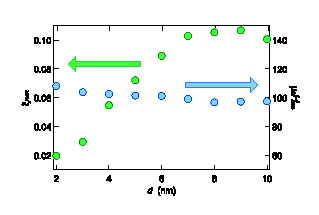
\includegraphics[width=9cm]{images/xi_Hreso_d_before.eps}
}
\caption{エッチングによりNi$_{81}$Fe$_{19}$の膜厚を変化させたときの$\xi_{\rm FMR}$及び$H_{\rm res}$.緑の円が$\xi_{\rm FMR}$を表し,青の円が$H_{\rm res}$を表している.
}
\label{fig:xi_Hreso_d_before} 
\end{figure}


Figure \ref{fig:xi_Hreso_d_before}を見ると$\xi_{\rm FMR}$が膜厚の減少に対して急激に変化している.またそれに対応して共鳴磁場$H_{\rm res}$も変化している.この傾向は他の試料でも再現しており,エッチングによりNi$_{81}$Fe$_{19}$の質が変化してしまっていると考えられる.エッチング前後の試料の光学カメラによる像がFig.\ref{fig:picture_before}である.

\begin{figure}[htbp]
\centerline{
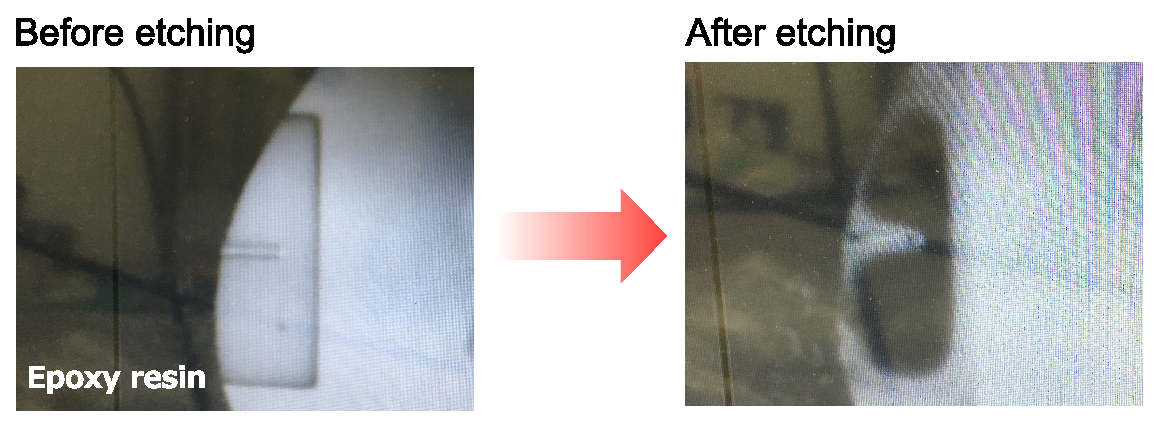
\includegraphics[width=9cm]{images/picture_before.eps}
}
\caption{Ni$_{81}$Fe$_{19}$/Pt二層薄膜のST-FMR試料の光学カメラ像.左の像がエッチング前,右の図がエッチング後の像である.エッチングにより試料から泡のようなものが出ているのがわかる.
}
\label{fig:picture_before}
\end{figure}

この像からわかるようにエッチングによりNi$_{81}$Fe$_{19}$薄膜から泡のようなものが吹き出している.またこの現象は同じゲート電圧を印可していても起きる頻度や量などが異なることから膜が均一に溶けていないことがわかる.

Fig.\ref{fig:xi_Hreso_d_before}の結果から$1/\xi_{\rm FMR}$と$1/d$の関係を計算することはできる.その結果がFig.\ref{fig:xi-1_before}である.

\begin{figure}[htbp]
\centerline{
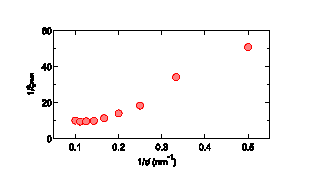
\includegraphics[width=9cm]{images/xi-1_before.eps}
}
\caption{Ni$_{81}$Fe$_{19}$/Pt二層薄膜のST-FMR試料の光学カメラ像.左の像がエッチング前,右の図がエッチング後の像である.エッチングにより試料から泡のようなものが出ているのがわかる.
}
\label{fig:xi-1_before}
\end{figure}

\textcolor{blue}{前章で述べたようにPtの$\xi_{\rm Dl}$及びの$\xi_{\rm FL}$の符号から,$1/\xi_{\rm FMR}$と$1/d$の傾きは負でなければならない.しかしFig.\ref{fig:xi_Hreso_d_before}において$H_{\rm res}$が変化し始めたあたりの膜厚から$1/\xi_{\rm FMR}$の傾きが正に転じている.}つまりこの膜厚付近からNi$_{81}$Fe$_{19}$が違う強磁性体になっている可能性がある.そのためST-FMR測定の設定が異なってしまっていると考えられる.この一つの原因としてあげられるのがNi$_{81}$Fe$_{19}$のNi及びFeの電気陰性度の違いによるエッチング速度の違いである.この差のためにNi$_{81}$Fe$_{19}$薄膜が一様にエッチングされず強磁性体がエッチングによってNi$_{81}$Fe$_{19}$ではないものに変化してしまっている可能性である.この可能性はXPSなどの元素分析で調べて検討しなければならない.\\

ここで再考したのがイオン液体に対するゲート電圧の方向である.通常の電気分解と比較して考える.粗銅の電気精錬を思い出すとFig. \ref{fig:denkibunkai}のように融解させたい物質(ここでは粗銅)を電圧の正側に接続している.

\begin{figure}[htbp]
\centerline{
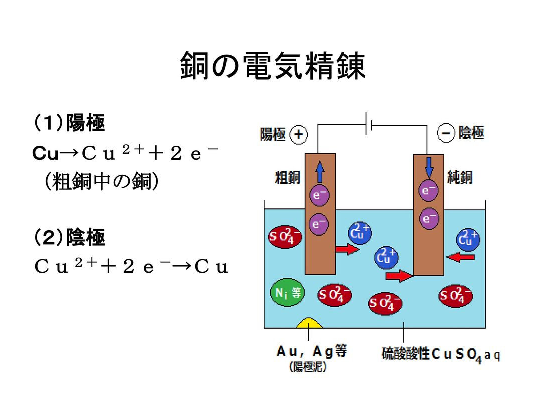
\includegraphics[width=9cm]{images/denkibunkai.eps}
}
\caption{粗銅の電気分解の模式図.溶ける粗銅が電圧の正側に接続している.
}
\label{fig:denkibunkai}
\end{figure}

ここまでの実験設定ではFig.\ref{fig:IL_resi_setup}のように融解させたい(エッチングしたい)試料側が電圧の負側に接続していた.しかしこの条件だと逆に電極側から(e$^{-}$)が引き抜かれ試料側に電子が集まってしまう.この設定でも,上で示したように試料を含んだ電気抵抗$R_{\rm AB}$が増加したことやFMRスペクトルの変化が観測されたことからNi$_{81}$Fe$_{19}$薄膜はエッチングされていたことは明らかである.しかし一方でこの設定では金属が電気化学効果によってイオン化して融解するという現象は起きてない可能性がある.そこで先行研究とはゲート電圧の印可方向が逆になってしまうが,試料側をゲート電圧の正側に接続して上記の実験と同様のエッチングプロセスを行なった.\\

\subsection{イオン液体による電気化学エッチング -負のゲート電圧-}


まずエッチングによりFig.\ref{fig:IL_resi_setup}の抵抗$R_{\rm AB}$がどのように変化するかを観測した.このとき用いた試料はNi$_{81}$Fe$_{19}$(8)/Pt(10)であり,エッチングプロセスはゲート電圧$3\rm\ V$を15 sec,待機時間をが240 secである.それを10シークエンス繰り返した.その結果がFig.\ref{fig:resichange_after}である.

\begin{figure}[htbp]
\centerline{
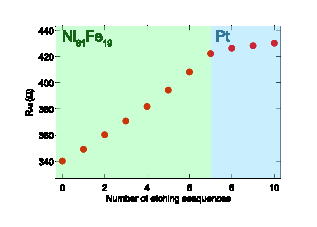
\includegraphics[width=9cm]{images/resichange_after.eps}
}
\caption{イオン液体による電気化学効果を利用したエッチングでの電気抵抗変化.緑の部分がNi$_{81}$Fe$_{19}$が青の部分がPtが溶けている部分だと考えられる.
}
\label{fig:resichange_after}
\end{figure}

Figure.\ref{fig:resichange_after}を見ると緑の領域と青の領域で抵抗変化率が異なっていることがわかる.ここから表面にあるNi$_{81}$Fe$_{19}$が溶け(緑の領域),表面にPtが現れるとPtが溶けることによって(青の領域)抵抗が増加していると推測できる.変化率の違いはNi$_{81}$Fe$_{19}$とPtの電気陰性度の違いを反映しており,Ni$_{81}$Fe$_{19}$よりPtの方が電気陰性度が小さいことと一致している.(\textcolor{blue}{ただしNi$_{81}$Fe$_{19}$の電気陰性度は一般的な合金の電気陰性度の算出の方法を参考にしている[].})

次にこの抵抗と同時に測定したST-FMR測定の結果をFig.\ref{fig:melting_after}に示した.ただしマイクロ波周波数を$7\rm\ GHz$,パワーを$100\rm\ mW$として行なった結果である.

\begin{figure}[htbp]
\centerline{
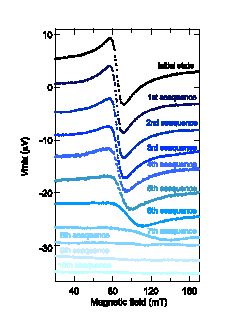
\includegraphics[width=8cm]{images/melting_after.eps}
}
\caption{イオン液体の電気化学効果によってNi$_{81}$Fe$_{19}$/Ptをエッチングした時のFMRスペクトルの変化.一番上のスペクトルが初期状態でそこからエッチングプロセスを繰り返した結果.
}
\label{fig:melting_after}
\end{figure}

このFig.\ref{fig:resichange_after}およびFig.\ref{fig:melting_after}の結果からゲート電圧方向を逆にしてもNi$_{81}$Fe$_{19}$の膜厚を削ることは可能なようである.むしろこのゲート電圧方向の方が均一にNi$_{81}$Fe$_{19}$薄膜がエッチングされているようである.このような推測は以下のような議論から考えられる.Figure.\ref{fig:melting_after}とFig.\ref{fig:meltingFMR_before}を比較すると共鳴磁場の変化が異なっている.前者はかなりエッチングが進行した後に共鳴磁場が変化しているのに対し,後者はエッチング初期から共鳴磁場のシフトが見られる.Ni$_{81}$Fe$_{19}$の膜厚を薄くすると飽和磁化が減少することは知られており[\textcolor{blue}{引用したほうがいい}],Fig.\ref{fig:melting_after}の共鳴磁場の変化はこの強磁性体も膜厚が極めて薄くなった影響を反映していると考えられる.対してFig.\ref{fig:meltingFMR_before}の結果はエッチングを始めた直後から共鳴磁場が変化しており,エッチングによるNi$_{81}$Fe$_{19}$の変化による共鳴磁場の変化も含まれると思われる.ここからゲート電圧の方向を負にした設定の方が強磁性薄膜が均一に溶けていると考えられる.

共鳴磁場の変化をFig.\ref{fig:resichange_after}の解析可能なスペクトルから算出するとFig.\ref{fig:Hreschange_after}の緑の円のようになる.またFMRスペクトルの周波数依存性から初期状態の飽和磁化$\mu_{0}M_{\rm s} = 664.29\rm\ mT$を出し,この初期状態の飽和磁化の値と共鳴磁場からKittelの式を用いてそれぞれの共鳴磁場に対応する飽和磁化を求めた値が\ref{fig:Hreschange_after}の青の円である.

\begin{figure}[htbp]
\centerline{
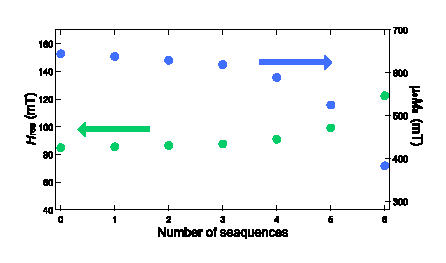
\includegraphics[width=10cm]{images/Hreschange_after.eps}
}
\caption{イオン液体の電気化学効果によってNi$_{81}$Fe$_{19}$/Ptをエッチングしたときの共鳴磁場及び飽和磁化の変化.
}
\label{fig:Hreschange_after}
\end{figure}

エッチングプロセスを7回以上繰り返すとFig.\ref{fig:resichange_after}の青の領域に入り,Fig.\ref{fig:melting_after}でもわかるようにFMRのスペクトルが観測できなくなる.上でも述べたように共鳴磁場がシークエンスの後半で大きく変化している.これはNi$_{81}$Fe$_{19}$の膜厚が薄くなることに連れて飽和磁化が小さくなることを示している.



ここでエッチングしたときの膜厚を求めたい.そのためにエッチング前と後のAFMを用いた試料の膜厚測定を行なった.その結果がFig.\ref{fig:AFMpicture}である.この測定から分かったバーの厚さは表\ref{table:AFM}のようになった.

\begin{figure}[htbp]
\centerline{
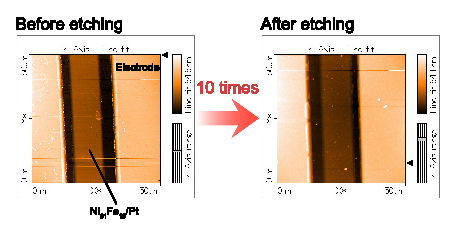
\includegraphics[width=11cm]{images/AFMpicture.eps}
}
\caption{エッチングプロセス前後のNi$_{81}$Fe$_{19}$/Pt薄膜試料のAFM像.像の中心にあるバー状のものが試料,それの周りにある部分が電極である.
}
\label{fig:AFMpicture}
\end{figure}


\begin{table}[hbtp]
  \caption{Ni$_{81}$Fe$_{19}$/Pt薄膜のエッチング前後の膜厚.Ptはほとんどエッチングされていないとすると}
  \label{table:AFM}
  \centering
  \begin{tabular}{lcr}
    \hline
           &   Before etching   & After etching  \\
    \hline \hline
    Ni$_{81}$Fe$_{19}$/Pt  & $17.03\rm\ nm$  & $9.63\rm\ nm$ \\
    \hline
  \end{tabular}
\end{table}

一方Fig.\ref{fig:resichange_after}からエッチングによる抵抗$R_{\rm AB}$の変化はわかる.この$R_{\rm AB}$には試料の抵抗だけでなく接触抵抗及び金電極の抵抗も含んでいる.Ni$_{81}$Fe$_{19}$/Pt二層薄膜の抵抗がそれぞれの層の抵抗$R_{\rm Ni$_{81}$Fe$_{19}$}$及び$R_{\rm Pt}$の並列回路で再現できると仮定し,試料以外の抵抗(接触抵抗及び金電極の抵抗など)を$R_{\rm ex}$とすると$R_{\rm AB}$は

\begin{eqnarray}
R_{\rm AB} = \frac{R_{\rm Ni_{81}Fe_{19}}R_{\rm Pt}}{R_{\rm Ni_{81}Fe_{19}}+R_{\rm Pt}} + R_{\rm ex}
\label{eq:RAB}
\end{eqnarray}
となる.この式\ref{eq:RAB}の関係に Ni$_{81}$Fe$_{19}$の厚さ$d$を含めて$d$を$R_{\rm AB}$で表したい.そのために個別で調べた表\ref{table:resi}の物性値を用いて$R_{\rm AB}$を$d$と$R_{\rm AB}$の関数とした式が式\ref{eq:RAB2}である.

\begin{table}[hbtp]
  \caption{Ni$_{81}$Fe$_{19}$およびPtの物性値.}
  \label{table:resi}
  \centering
  \begin{tabular}{ccc}%lが左cが中央rが右揃えって意味
    \hline
           &   Ni$_{81}$Fe$_{19}$   & Pt  \\
    \hline \hline
   electrical resistivity  & $1.057\times10^{-6}\rm\ \Omega\cdot m$  & $3.00\times10^{-7}\rm\ \Omega\cdot m$\\
   thickness  &  $d\rm\ nm$  &  $10\rm\ nm$\\
   length  &  $130\rm\ \mu m$  &  $130\rm\ \mu m$\\
   width  &  $10\rm\ \mu m$   &  $10\rm\ \mu m$\\
    \hline
  \end{tabular}
\end{table}


\begin{eqnarray}
R_{\rm AB} = \frac{1}{\frac{1}{390}+7.277\times10^{4}d} + R_{\rm ex}
\label{eq:RAB2}
\end{eqnarray}

まず測定結果から$R_{\rm AB}$の値を求めて式\ref{eq:RAB2}から取り除きたい.そうすれば$d$が$R_{\rm AB}$だけの関数になり,Fig.\ref{fig:resichange_after}の結果からそれぞれのNi$_{81}$Fe$_{19}$の膜厚が見積れる.
Figure.\ref{fig:resichange_after}の緑と青の領域の境界でNi$_{81}$Fe$_{19}$の膜厚が$0\rm\ nm$になったと仮定すると,この境界における抵抗$R_{\rm AB}(d=0\rm\ nm)$はPtと$R_{\rm ex}$だけで表せる.表\ref{table:resi}の物性値を用いたPt単層の抵抗は$390\rm \Omega$になるはずだが,$R_{\rm AB}(d=0\rm\ nm) = 422.09\rm\ \Omega$である.この差$422.09-390 = 32.09\rm\ \Omega$が$R_{\rm ex}$と考えられる.この$R_{\rm ex}$はエッチングによって変化しないと考えられるので,$R_{\rm ex}$をFig.\ref{fig:resichange_after}の全体の測定結果から引く.その結果がFig.\ref{fig:RAB-Rex}である.


\begin{figure}[htbp]
\centerline{
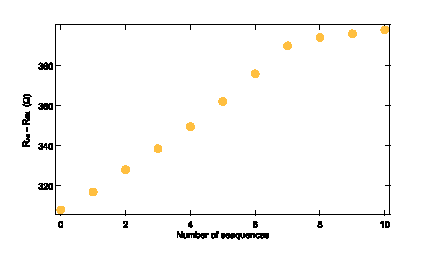
\includegraphics[width=9cm]{images/RAB-Rex.eps}
}
\caption{$R_{\rm AB}-R_{\rm ex}$のエッチングによる変化.
}
\label{fig:RAB-Rex}
\end{figure}

式\ref{eq:RAB2}を変形すると式\ref{eq:d}となる.

\begin{eqnarray}
d = \frac{1}{7.277\times10^{4}}\left(\frac{1}{R_{\rm AB} - R_{\rm ex}}-\frac{1}{390}\right)
\label{eq:d}
\end{eqnarray}
この計算をFig.\ref{fig:RAB-Rex}に適応し$d$を求めたのがFig.\ref{fig:d_after}である.

\begin{figure}[htbp]
\centerline{
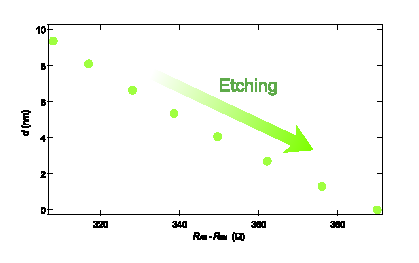
\includegraphics[width=9cm]{images/d_after.eps}
}
\caption{$R_{\rm AB}-R_{\rm ex}$から計算した$d$.シークエンス7以降はNi$_{81}$Fe$_{19}$が溶けた後なので示していない.
}
\label{fig:d_after}
\end{figure}

こうして見積もった膜厚$d$と$\xi_{FMR}$の関係をプロットしたものがFig.\ref{fig:xi-1_after}である.この傾き及び切片から$\xi_{\rm DL}$及び$\xi_{\rm FL}$が算出できる.

\begin{figure}[htbp]
\centerline{
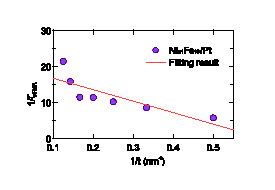
\includegraphics[width=10cm]{images/xi-1_after.eps}
}
\caption{イオン液体の電気化学効果を用いて求めた$\xi_{\rm FMR}^{-1}$と$t^{-1}$の関係.
}
\label{fig:xi-1_after}
\end{figure}

Figure.\ref{fig:xi-1_after}から見積もった$\xi_{\rm DL}$及び$\xi_{\rm FL}$を表\ref{table:xi}に示した.比較対象として本研究室で異なるNi$_{81}$Fe$_{19}$の膜厚を持った試料を作成し定量した値と他のグループが定量した値を記載した.


\begin{table}[hbtp]
  \caption{Ni$_{81}$Fe$_{19}$/Ptの$\xi_{\rm DL}$及び$\xi_{\rm FL}$.}
  \label{table:xi}
  \centering
  \begin{tabular}{ccc}%lが左cが中央rが右揃えって意味
    \hline
           &   $\xi_{\rm DL}$   & $\xi_{\rm FL}$  \\
    \hline \hline
   Etched with IL  & $0.0347 $  & $-0.322$\\
   Prepared each samples  &    &  \\
   \textcolor{blue}{Reference[]}  & $0.100\pm 0.005$  & $-0.004\pm 0.003$\\
    \hline
  \end{tabular}
\end{table}


表\ref{table:xi}でわかるように$\xi_{\rm DL}$及び$\xi_{\rm FL}$は膜厚を変えた試料を複数用意して定量した値と本研究の結果とでそれぞれ誤差がある.$\xi_{\rm DL}$はFig.\ref{fig:xi-1_after}における切片の逆数と同値である.エッチング初期におけるフィッティング誤差が大きく影響を及ぼしていると考えられる.また膜厚を算出する際に抵抗率が一定であるという過程を用いている.\textcolor{blue}{しかし実際は膜厚が薄くなるにつれて薄膜の表面散乱の影響が大きくなり低効率の増加が見られる[].}その効果を無視している影響も考えられる.



\section{まとめ}
本研究で得られた主要な結果は以下の2点である。
\begin{enumerate}
 \item Ni$_{81}$Fe$_{19}$/Pt二層薄膜におけるST-FMR測定の強磁性体膜厚依存性を測定した.
 \item イオン液体の電気化学効果を用いたエッチング方法を確立し,単一の試料を用意するだけでST-FMR測定の強磁性体膜厚依存性を測定可能にした.
\end{enumerate}

\chapter{SLG/Al$_{2}$O$_{3}$基板におけるコバルトインターカレーション}

本章ではグラフェンにおけるスピン軌道相互作用の増大を目指し,グラフェン/サファイア基板におけるコバルトのインターカレーションの研究についてまとめる.
まず化学蒸着(CVD:chemical vapor deposition)法によってSLGを作成した結果及びコバルトの蒸着について述べる.その後作成したSLGの質を評価した結果をまとめる.最後にコバルトインターカレーションについての結果を述べる.第\ref{chap:intro}章の\pageref{subsec:graphene}ページの\ref{subsec:graphene}で述べたように本研究ではCVD法を用いてグラフェンを作成した.まずこれについて述べる.

\section{CVD法によるSLGの作成及びコバルトのEB蒸着}
\subsection{CVD法によるSLG成長}
ここでは本研究で用いたSLGの作成について述べる.まず(0001)面Al$_{2}$O$_{3}$基板をダイアモンドペンを用いて$1\rm\ cm \times 1\rm\ cm$に切り分けた.この$1\rm\ cm \times 1\rm\ cm$のAl$_{2}$O$_{3}$基板の表面の有機物をクリーニングするために大気中で900$\rm\ C^{\circ}$を保ち6時間アニールをした.CVDを行うガラス管はFig.\ref{fig:CVD}のような形状である.

\begin{figure}[htbp]
 \begin{center}
  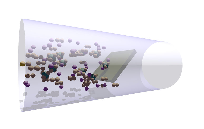
\includegraphics[width=100mm]{images/CVD.eps}
 \end{center}
 \caption{CVD法の概略図.緑の球が炭素,オレンジの球が水素,紫の玉がアルゴンを示している.}
 \label{fig:CVD}
\end{figure}

このガラス管の中にAl$_{2}$O$_{3}$基板を用意し,内部を$1.6\times10^{-5}\rm\ Pa$の真空にする.そこで内部の空間及び基板表面の有機物を取り除くために300$\rm\ C^{\circ}$で1時間アニールした.その後菅内部の温度を1時間ほどかけて1000$\rm\ C^{\circ}$にし,安定に1000$\rm\ C^{\circ}$になった時にメタノールガスを流す.そこで真空をひくポンプ(ターボ分子ポンプ)から切り離しCVD用のポンプ(ロータリーポンプ)だけで菅の真空を引き始める.これにより内部圧力が上がり$2.6\times10^{2}\rm\ Pa$ほどで定常状態になる.内部圧力の増加によりCVDに必要な化学反応が始まる.その後4時間1000$\rm\ C^{\circ}$を保持しCVDを行なった.4時間経過した直後にCVDによるグラフェンの成長を止めるためターボ分子ポンプによる真空引きを開始し,同時にドライヤーを用いて急冷した.この急冷の温度勾配が重要である.急冷によって基板における化学反応の停止及び炭素の結合を促すと考えられている.そのためできるだけ素早く行なった.CVDが終わった直後の菅内部の圧力は$2.0\times10^{2}\rm\ Pa$となっていた.
CVDが終わったあとにこの後に述べるラマン分光法によりグラフェンが実際に成長しているかどうかを確認し,その質を評価した.その後グラフェンの成長が確認できた試料にコバルトを蒸着した.

\subsection{SLG/Al$_{2}$O$_{3}$におけるコバルト蒸着}

SLG上にコバルトを蒸着するためにEB(electron beam)蒸着法を用いた.EB蒸着法とは電子線を用いて金属ターゲットを加熱することでそれを蒸発させて基板に金属薄膜を形成する方法である.金属薄膜を作成する方法は他にも存在するがスパッタリング法のような蒸着する金属分子のエネルギーが高い方法はグラフェンを傷つけてしまい欠陥が生まれてしまう.それを避けるためにEB蒸着法を選択した.
蒸着チャンバーにSLG/Al$_{2}$O$_{3}$試料を入れSLGのクリーニングのため600$\rm\ C^{\circ}$にして20 min加熱した.加熱することによりSLGに付着した有機物が蒸発しチャンバー内部の圧力が増加する.その圧力が$10^{-6}\rm\ Pa$程度になった時にクリーニングを終えた.その後コバルトのレートが$0.05\rm\ \AA/sec$で一定になるようにフィラメント電流を24 mAにし,定常状態になってから蒸着を開始しコバルトをSLG/Al$_{2}$O$_{3}$上に2原子層蒸着した.

\subsection{Co/SLG/Al$_{2}$O$_{3}$のアニールによるインターカレーション}
インターカレーションは試料を加熱することにより分子が他の分子組織に入り込む現象である.そのため他のグループを参考にし真空中でアニールをすることによりコバルトをSLG/Al$_{2}$O$_{3}$界面にインターカレートさせようと考えた.
真空中で基板を加熱することによりインターカレーションを目指した.実際には600$\rm\ C^{\circ}$から800$\rm\ C^{\circ}$までアニール温度を変えてインターカレーションが起こる温度を探索した.温度はパイロメータで測定した温度に対応している.
\begin{table}[htbp]
 \caption{インターカレーションアニールの条件.}
 \begin{center}
  \begin{tabular}{ccc}\toprule
  基板加熱装置の温度計 (C$^{\circ}$)	&	パイロメータの温度表示	(C$^{\circ}$)	&	真空度 (Pa)	\\	\hline 
	562		&	392 			&	$1.8\times10^{-7}$\\
	620   &   565      &  $3.0\times10^{-7}$  \\
	768  &	712			&	$2.1\times10^{-6}$	\\
	893  &   820  &    $5.2\times10^{-6}$     
						\\	\bottomrule
  \end{tabular}
 \end{center}
 \label{tb:ICcond}
\end{table}

基板加熱装置にも温度計が付いているがその温度計は基板ホルダーの温度を示しているため,実際の基板の温度とは乖離している.その温度とアニールした時のチャンバー内の圧力は表\ref{tb:ICcond}にまとめた.

\section{ラマン分光法によるSLGの評価}
\subsection{ラマン分光法について}
次にAl$_{2}$O$_{3}$上にグラフェンが成長しているのかを確認するために行ったラマン分光測定の原理及びその結果について述べる.

ラマン分光とは光の非弾性散乱である.光の散乱の前後でエネルギーが変化しないものをレイリー散乱という.レイリー散乱では光の電場が分子の中で振動する双極子モーメントが発生し,その双極子モーメントの振動によって電場が新たに生成され散乱が起きる.一方その双極子モーメントが分子振動を引き起こすことがある.これは電子-格子相互作用を介し双極子モーメントのエネルギーの一部が分子振動に受け渡される.つまりこの時,双極子モーメントの振動によって発生する光のエネルギーは分子振動のエネルギー分だけ減少している.これがラマン効果である.格子振動は量子化されその振動数を$\omega$とするとラマン散乱光のエネルギーは入射した光のエネルギーから$\hbar\omega$を差し引いたエネルギーを持つ.この散乱光をCCDカメラなどで測定すると入射光のエネルギーから$\hbar\omega$だけずれたエネルギー(ラマンシフト)において強い散乱光強度を得られる.これをラマンスペクトルと呼び,分光された各波長の情報を波数(cm$^{2}$)に換算しFig.\ref{fig:ramanshift}のようなスペクトルにする.

\begin{figure}[htbp]
\centerline{
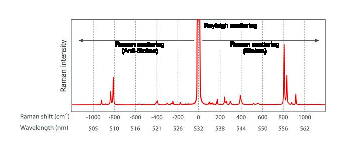
\includegraphics[width=12cm]{images/ramanshift.eps}
}
\caption{ラマンシフトの例.
}
\label{fig:ramanshift} 
\end{figure}
レイリー散乱は弾性散乱のためエネルギー損失がなく散乱しエネルギーシフトは起きない.ラマンシフトがレイリー散乱のスペクトルから長波長側及び短波長側に観測されていることがわかるが,これは双極子モーメント振動から分子振動にエネルギーを与える(長波長側)だけでなく双極子モーメントが分子振動からエネルギーをもらう(短波長側)の散乱過程も可能なためである.これはそれぞれストークス線,及びアンチストークス線と呼ばれる.実際は強度の強いストークス線を用いて解析される.
格子振動数$\omega$は分子の種類や結合状態によって異なるため,ラマンスペクトルを測定することで分子の状態や構造に関する情報を手に入れることができる.横軸は分子の振動情報(結合状態や電子状態),縦軸の比は活性の強さを反映している.




ラマン散乱効果では入射光の波長は関係ないが,入射光のエネルギーがラマンスペクトルを得たい物質の吸収エネルギーに一致する場合はラマン強度は著しく強くなる.このとき共鳴ラマン分光という.第\ref{chap:intro}章における\pageref{sec:graphene}で述べたようにグラフェンは可視光付近の光に対して光吸収を伴うため,可視光に対してグラフェンは常に共鳴ラマン分光となる.この効果のためにグラフェンは一層($0.335\rm\ nm$)であってもラマン分光が観測できる.またFig.\ref{fig:ramanshift}からもわかるように散乱光のほとんどはレイリー散乱による光であり.レマン散乱光はレイリー散乱の$10^{-6}$程度であるため実際の光源は強度の強いレーザー光を用いた.

\subsection{ラマンスペクトルの測定結果}
次にAl$_{2}$O$_{3}$基板上にCVD法によってSLGが成長できたかを確認するためにラマン分光測定を行なった結果を述べる.比較対象として転写法を用いてSiO$_{2}$基板上に作成したSLGのラマンスペクトルを載せた.その結果がFig.\ref{fig:raman_init}である.
\begin{figure}[htbp]
\centerline{
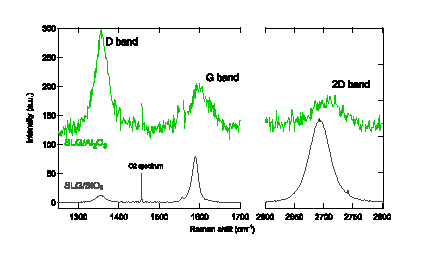
\includegraphics[width=12cm]{images/raman_init.eps}
}
\caption{SLG/SiO$_{2}$およびSLG/Al$_{2}$O$_{3}$のラマンスペクトル.
}
\label{fig:raman_init} 
\end{figure}

SiO$_{2}$上のグラフェンのラマン散乱光は増強されることが知られグラフェンの一般的なラマンシフトを示すのに適している.Figure.\ref{fig:raman_init}の灰色の線で示したSLG/SiO$_{2}$のスペクトルのようにグラフェンに特有なバンドは3つある.一つは$1580\rm\ cm^{-1}$付近にあるGバンドである.これはsp$^{2}$混成軌道に共通されるバンドである.また$2700\rm\ cm^{-1}$付近にある2Dバンドもグラフェン特有である.これは散乱時のグラフェン内のディラックコーンの電子の励起における二重共鳴ラマン効果により生じる.$1350\rm\ cm^{-1$付近に存在するDバンドはグラフェンの欠陥により生じるバンドである.DとGバンドの比はグラフェンの結晶性にほぼ比例すると知られている.また一般的に2DバンドとGバンドの比はグラフェンの層数に比例している.層数が増加するほどGバンドに対する2Dバンドの強度は小さくなる.1層の時は2Dバンドの方が大きく2層以上になるとGバンドの方が大きくなる.

SLG/SiO$_{2}$と比較してSLG/Al$_{2}$O$_{3}$のDバンド/Gバンドの比は大きくなっている.これは酸化物上におけるSLGの成長が難しいことを示している.しかしGバンド及び2Dバンドの存在からAl$_{2}$O$_{3}$上にSLGを成長させることに成功したことがわかる.2DバンドがGバンドより小さいのはグラフェンの層数が2層である可能性,もしくはキャリアドープの効果が考えられる\textcolor{blue}{[ドープの論文]}.実際,グラフェンが成長した表面に二層目のグラフェンが成長することは難しくCVDが進行しないことが考えられるため,この結果からAl$_{2}$O$_{3}$との結合によりグラフェンの電子状態がSiO$_{2}$上に成長している時とは異なっていることが予想される.
ノイズが大きく見えるのはSLG/SiO$_{2}$のラマンスペクトル強度が増強されているためにノイズが潰れていて,対照的にSLG/Al$_{2}$O$_{3}$のノイズが大きいように見える.

Al$_{2}$O$_{3}$上にSLGが成長しているのが確認できた.次にこの試料を用いてコバルトインターカレーションの実現を目指した.


\section{コバルトインターカレーションの評価}
コバルトがSLG/Al$_{2}$O$_{3}$界面にインターカレートすることを観測するために選択した方法がXPS測定の角度依存性を用いた方法である.XPSとはX線光電子分光(X-ray Photoelectron Spectroscopy)法の略語であり,その名の通りX線を用いて原子軌道の電子を光電子として励起させ,その光電子のエネルギーから原子の種類や状態を測定する方法である.その概略図をFig.\ref{fig:XPS_concept}に描いた.

\begin{figure}[htbp]
\centerline{
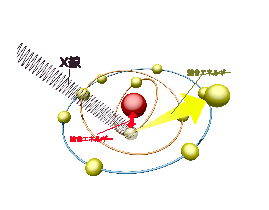
\includegraphics[width=12cm]{images/XPS_concept.eps}
}
\caption{XPS測定の概要図.X線が原子に入射した時その入射エネルギー$h_{\nu}$が電子の結合エネルギー$E_{\rm B}$以上だと電子を結合状態からはじき出し光電子として放出する.その光電子の持っているエネルギー$E_{\rm k}$から原子の電子状態や構造が解析できる.
}
\label{fig:XPS_concept} 
\end{figure}

原子にエネルギー$h_{\rm\nu}$を持ったX線を照射すると原子内部の結合エネルギー$E_{\rm B}$で核に束縛された電子が励起され,運動エネルギー$E_{\rm K}$を持った光電子として飛び出す.その光電子の$E_{\rm K}$は物質の仕事関数$\phi$を用いて

\begin{eqnarray}
E_{\rm K} = h_{\rm\nu} - E_{\rm B} -\phi
\label{eq:XPS1}
\end{eqnarray}
と表せる.ここから式を変形すると
\begin{eqnarray}
E_{\rm B} = h_{\rm\nu} - E_{\rm K} -\phi
\label{eq:XPS2}
\end{eqnarray}
となる.このとき照射したX線のエネルギーは自身で決定し仕事関数は求めることができるので既知である.つまり光電子の運動エネルギーを測定することで光電子を束縛していた結合エネルギーの値を定量することができる.結合エネルギーは物質と軌道の組み合わせに対して一対一対応しているため,結合エネルギーを定量することでX線を照射した表面に存在する物質を調べることができる.
またX線の侵入長が数nmであることからXPSは表面敏感な測定である.このことを利用しXPS測定の角度依存性を用いることによって表面付近の元素分布の深さ分解を定量することができる.
\begin{figure}[htbp]
\centerline{
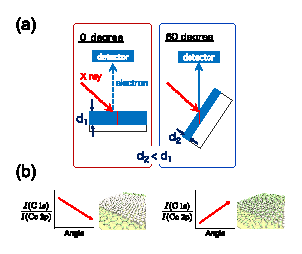
\includegraphics[width=10cm]{images/XPSAng_concept.eps}
}
\caption{XPS測定の角度分解の概要図.(a)X線の入射角が0度のときと60度のときを比較すると,60度のときの方がX線の侵入深さが浅くなっている.このように試料のX線に対する傾きを変化させることによって角度分解を行なった.(b)炭素とコバルトの強度比$I(\rm C\ 1s)/I(\rm Co\ 2p)$の角度に対する振る舞いによって再表面にある物質を同定づることが可能である.
}
\label{fig:XPSAng_concept} 
\end{figure}

Figure.\ref{fig:XPSAng_concept}(a)のようにX線の入射角を深くするとX線によって励起される原子の深さが浅くなる.つまり角度をつければつけるほどより表面敏感になる.これを用いることによって深さ方向の物質分布を定量することができる.XPSの角度分解を利用することによって,コバルトがインターカレートしていない場合Co/SLGの順番なので角度を浅くしていくとコバルトの強度が相対的に増加していくはずである.逆にコバルトがSLGの下に潜った場合,SLG/Coなので角度を増加していくと炭素の強度が増加していく.Fig.\ref{fig:XPSAng_concept}(b)に示すように,コバルトの強度を$I(\rm Co\ 2p)$,炭素の強度を$I(\rm C\ 1s)$と表すと,角度に対しての振る舞いが逆になるはずである.
実際の実験の流れはコバルトをSLG/Al$_{2}$O$_{3}$上に蒸着した試料をアニールし,その試料のXSP測定の角度分解を行い,その後再度アニール温度を変えて試料を焼くことを繰り返した.この工程は全て真空中で行なった.ただしアニールは$10^{-6}\rm\ Pa$,XPS測定は$10^{-7}\rm\ Pa$台の下で行なった.

\subsection{XPS測定}
では実際のXPS測定の結果を述べる.
XPS測定で得られる生に得られるデータはある運動エネルギーを持った光電子がどれだけ検出されたかというものである.スペクトルは横軸が光電子の運動エネルギー(eV)であり縦軸がその運動エネルギーを持った光電子の検出されたカウント数(counts/sec)である.しかし実際に物質の種類などを同定するために必要な値は運動エネルギーではなく結合エネルギーである.そこで式\ref{eq:XPS2}を用いて運動エネルギーを結合エネルギーに変換しなくてはならない.本研究ではXPSにおけるX線源としてMgK\alpha を用いているためX線のエネルギーは1253.6 eVである.エミッションカレントは10.0 mAに一定しにて電圧は100 kVとした.パスエナジーは50に設定した.あと必要な値は仕事関数$\phi$である.ここで今回のような絶縁体(半導体などの導電性の低い材料)を取り扱う場合,実際問題としてXPS測定は中性のX線を照射し負に帯電している電子を放出させているため試料が正に帯電してしまう.この帯電(チャージアップ)のため仕事関数とは別に光電子に対するエネルギー障壁が増加する.この仕事関数とチャージアップの影響を含めたエネルギー障壁を$\Phi$とすると式\ref{eq:XPS2}における$\phi$を$\Phi$に書き換えられる.この分まで補正するために通常は試料の基板に含まれる元素(試料の変化に伴って状態が変化しないものを選択する)のスペクトルピークで補正をかける.今回の研究では基板に含まれるAlを基準とした.例えばAl2pのピークだとわかるスペクトルのピーク位置が86 eVだとする.式\ref{eq:XPS2}を考えて,まずX線のエネルギーから運動エネルギーである86 eVを引くと,$E_{\rm B}+\Phi = 1253.6-86=1167.6\rm\ eV$となる.実際のAl2pの結合エネルギーは$74.7\rm\ eV$なので,$\Phi = 1167.6 - 74.7 = 1092.9\rm\ eV$となる.つまり得られた生データの横軸である光電子の運動エネルギー$E_{\rm K}$から$E_{\rm B}$を求めるためには

\begin{eqnarray}
E_{\rm B} = 1253.6 - E_{\rm K} -1092.9 = 160.7 -E_{\rm K}
\label{eq:XPS3}
\end{eqnarray}
という変換をすれば結合エネルギーを得られる.ただし物質の仕事関数は一定であるがチャージアップは測定するたびに装置の状況(真空度など)や測定環境(温度や湿度)によって変化するため,アニールした後などXPS測定チャンバーから移動するたびに補正項$\Phi$を計算した.以上の補正をして得られた600$\rm\ C^{\circ}$でアニールしたCo/SLG/Al$_{2}$O$_{3}$についてのXPSスペクトルがFig.\ref{fig:600aneal_1st_0deg}である.
\begin{figure}[htbp]
\centerline{
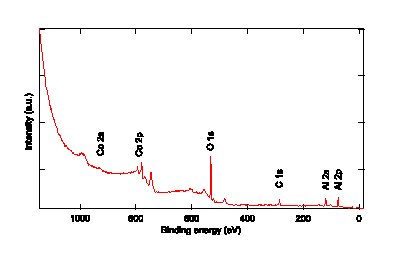
\includegraphics[width=12cm]{images/600aneal_1st_0deg.eps}
}
\caption{600$\rm\ C^{\circ}$でアニールしたCo/SLG/Al$_{2}$O$_{3}$のXPSスペクトル.コバルト,炭素及びAl$_{2}$O$_{3}$のアルミニウムと酸素のピークが見える.他のピークが見られないことから不純物のコンタミが少ないと考えられる.
}
\label{fig:600aneal_1st_0deg} 
\end{figure}

これはワイドスキャンと呼ばれ,表面に存在する元素を網羅的に確認するために行った.しかしこのワイドスキャン時は大雑把に把握するのが目的のためステップ数を荒く設定した.ワイドスキャン後に詳細に定量したい元素のピーク付近のナロースキャンを行なった.XPS測定時の設定を参考のために表\ref{tb:XPScondition}にまとめた.
\begin{table}[htbp]
 \caption{XPS測定時の条件設定}
 \begin{center}
  \begin{tabular}{cccc}\toprule
  	スキャン	&	ステップ幅(eV)	&	パスエナジー		&	積算回数	\\	\hline
	ワイド(全体を網羅的)	&	1.007		&	100	&	10				\\
	Al2p&	0.061		&	50		&	70
	\\
	C1s&  0.061  &    50  & 400
	\\
	Co2p& 0.061  &   50   &   100
						\\	\bottomrule
  \end{tabular}
 \end{center}
 \label{tb:XPScondition}
\end{table}

ただしステップ数は測定点間隔を表す.パスエナジーとは,運動エネルギー$E_{\rm\ B}$からパスエナジーだけずれたエネルギーを持つ光電子を$E_{\rm\ B}$になるように加速・減速させてXPS装置の検出器に入れる.つまりパスエナジーが大きいほど検出強度(検出される光電子数)は大きくなるがその分誤差は大きくなる.また積算回数は600$\rm\ C^{\circ}$でアニールした際の値であり,測定ごとに解析に十分なスペクトル形状となるような値を選んだ.(Coがインターカレートした際には炭素がコバルトの上にあるためコバルトの強度が弱くなるのでその分コバルトの積算回数を大きくした.)コバルトとグラフェン由来の炭素及びAl$_{2}$O$_{3}$基板のアルミニウムと酸素のピークが見える.ここからは他の物質のコンタミは確認できなかった.

次にFig.\ref{fig:600aneal_1st_0deg}のナロースキャンの結果をFig.\ref{fig:600aneal_1st_0deg_narrow}に示す.

\begin{figure}[htbp]
\centerline{
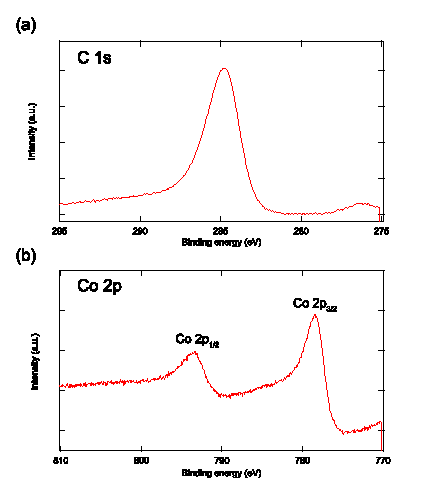
\includegraphics[width=10cm]{images/600aneal_1st_0deg_narrow.eps}
}
\caption{600$\rm\ C^{\circ}$でアニールしたCo/SLG/Al$_{2}$O$_{3}$のC1s(a)及びCo2p(b)のピーク.(b)コバルトの2p軌道はスピン軌道相互作用によって2p$_{1/2}$と2p$_{3/2}$の2準位に分裂している.
}
\label{fig:600aneal_1st_0deg_narrow} 
\end{figure}

コバルトの2p軌道はスピン軌道相互作用により縮退がとけ2p$_{1/2}$と2p$_{3/2}$の二つのピークが存在する.以上の結果は試料に対しX線は垂直(0度)に照射している.インターカレートが起きている確認するために炭素とコバルトの強度比$I(\rm C\ 1s)/I(\rm Co\ 2p)$を求める.この強度として本研究ではスペクトルの面積を用いた.コバルトは2p$_{3/2}$のピーク面積をその強度として用いた.このときこの600$\rm\ C^{\circ}$でアニールしたCo/SLG/Al$_{2}$O$_{3}$の0度の時の炭素とコバルトの強度比は$I(\rm C\ 1s)/I(\rm Co\ 2p) = 3.35$であった.
0度の時と同様の測定をX線の試料に対する照射角度を60度にして行なった.そのときの炭素とコバルトの強度比は$I(\rm C\ 1s)/I(\rm Co\ 2p) = 2.74$であった.角度を増加させると炭素に対するコバルトの強度が増加しているこの結果は表面にコバルトが多く存在していることを示している.つまり600度アニールではコバルトのインターカレーションは起きていないことがわかる.

次に同じ試料をアニールのチャンバーに移し700度のアニールをして再度XPS測定を行なった.その結果のワイドスキャン及びC1s,Co2pのスペクトルをFig.\ref{fig:700aneal_1st}に示す.

\begin{figure}[htbp]
\centerline{
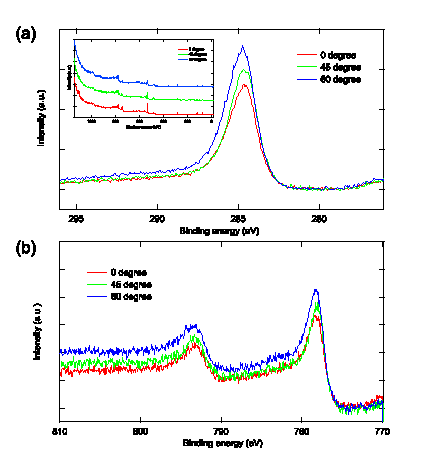
\includegraphics[width=10cm]{images/700aneal_1st.eps}
}
\caption{700$\rm\ C^{\circ}$でアニールしたCo/SLG/Al$_{2}$O$_{3}$のC1s(a)及びCo2p(b)のピーク.インセットはワイドスキャンを示している.
}
\label{fig:700aneal_1st} 
\end{figure}

この結果からピーク面積を求めてその炭素とコバルトの強度比は$I(\rm C\ 1s)/I(\rm Co\ 2p)$を定量した.その結果をFig.\ref{fig:rate_comparison}に示す.

\begin{figure}[htbp]
\centerline{
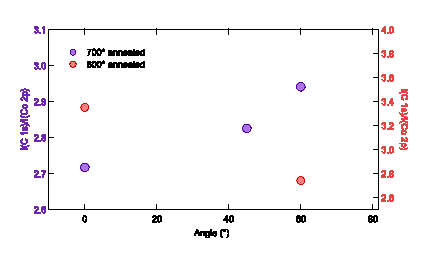
\includegraphics[width=10cm]{images/rate_comarison.eps}
}
\caption{600$\rm\ C^{\circ}$及び700$\rm\ C^{\circ}$でアニールしたCo/SLG/Al$_{2}$O$_{3}$の炭素とコバルトの強度比$I(\rm C\ 1s)/I(\rm Co\ 2p)$の角度依存性.
}
\label{fig:rate_comparison} 
\end{figure}

XPS測定はX線の照射角度が大きくなるほど,より表面敏感な測定になるためFig.\ref{fig:rate_comparison}の600$\rm\ C^{\circ}$アニールの結果のように$I(\rm C\ 1s)/I(\rm Co\ 2p)$の比が角度に対して小さくなっていくのは表面にコバルトが存在していることを表している.対してFig.\ref{fig:rate_comparison}における700$\rm\ C^{\circ}$アニールの結果のように角度を大きくしていくほど$I(\rm C\ 1s)/I(\rm Co\ 2p)$の比が増加してくのは,表面にコバルトより炭素が多くあることを示している.つまりCo/SLG/Al$_{2}$O$_{3}$を700$\rm\ C^{\circ}$でアニールすることによってコバルトがSLG/Al$_{2}$O$_{3}$界面にインターカレートしたことを示唆している.

コバルトのインターカレーションをさらに確認するために試料を大気中に取り出した後の試料を再度XPS測定した.というのも,もしコバルトがSLG/Al$_{2}$O$_{3}$界面にインターカレートしていた場合SLGが酸化防止膜として働き,界面に存在するコバルトが参加しないことが予想される.一方コバルトがSLGの上に存在していた場合はコバルトが酸化されるはずである.酸化コバルトにおける2p軌道の電子状態は酸素との結合によりコバルトにおけるものから変化しているため,XPS測定で判別できる.もっともわかりやすい変化は,コバルトの2p$_{1/2}$ピークと2p$_{3/2}$ピークの差$\Delta_{\rm Co2p}$の変化である.コバルトは$\Delta_{\rm Co2p} = 15.05\rm\ eV$であるが,酸化コバルトCoOでは$\Delta_{\rm Co2p} = 10.5\rm\ eV$となる.そこで700$\rm\ C^{\circ}$アニールをした後大気暴露した場合コバルトが酸化するかを確認するために,SLG/Al$_{2}$O$_{3}$上にコバルトを蒸着した試料を700$\rm\ C^{\circ}$アニールしたものとアニールをしなかったものを大気にさらしその後真空中に戻しXPS測定行ない,コバルトの2p軌道の電子状態を観測した.その結果がFig.\ref{fig:atom_comparison}である.

\begin{figure}[htbp]
\centerline{
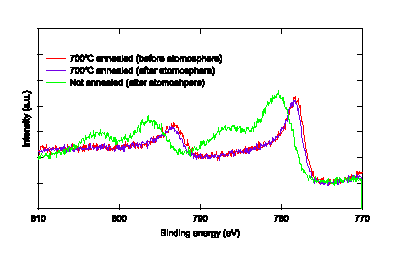
\includegraphics[width=12cm]{images/atom_comparison.eps}
}
\caption{Co/SLG/Al$_{2}$O$_{3}$のCo2pピーク.赤のスペクトルは700$\rm\ C^{\circ}$アニールして大気に出さずXPS測定をしたもの.紫のスペクトルは700$\rm\ C^{\circ}$アニールした後大輝暴露し,再度真空中に戻しXPS測定をした試料.緑のスペクトルはコバルトをSLG/Al$_{2}$O$_{3}$上に蒸着した後アニールをせず大気暴露し,その後真空に戻しXPS測定した試料.
}
\label{fig:atom_comparison} 
\end{figure}

比較対象として700$C^{\circ}$アニールした後に大気暴露せずにXPS測定した結果(赤のスペクトル,Fig.\ref{fig:700aneal_1st}(b)における0degの結果と同様.)も載せてある.この結果を見ると700$C^{\circ}$アニールした試料は大気暴露後も大気に出す前のスペクトルとほとんど変化していない.一方アニールをせずに大気暴露した試料はスペクトル形状が変化していて,$\Delta_{\rm Co2p}$も増加している.$\Delta_{\rm Co2p}$をそれぞれ表\ref{tb:atom_comparison}にまとめた.

\begin{table}[htbp]
 \caption{Fig.\ref{fig:atom_comparison}における$\Delta_{\rm Co2p}$}
 \begin{center}
  \begin{tabular}{cc}\toprule
  	試料	&	$\Delta_{\rm Co2p}$	eV	\\	
  	\hline
	700$C^{\circ}$ annealed	(before atomosphere)&	15.08						\\
	700$C^{\circ}$ annealed	(after atomosphere)&	15.20		
	\\
	Not annealed (after atomosphere)&  15.56  
						\\	\bottomrule
  \end{tabular}
 \end{center}
 \label{tb:atom_comparison}
\end{table}




さらにアニールをしていない試料は2p$_{1/2}$ピークと2p$_{3/2}$ピークそれぞれの高エネルギー側にサテライトピークが存在している.これらからアニールをせずに大気暴露した試料はコバルトが酸化していると言える.これらの結果からアニールをした試料のコバルトだけが大気暴露しても酸化しないことが分かった.これはアニールしたことによってコバルトがSLGの下に入り込みSLGの酸化防止膜の効果によって酸化が防がれていることを示唆している.

これらの試料についてラマン分光測定をした.次にその結果について述べる.

\subsection{ラマン分光測定}

Co/SLG/Al$_{2}$O$_{3}$をアニールすることでSLGの電子状態が変化していないかを確認するためにCo/SLG/Al$_{2}$O$_{3}$を700 C$^{\circ}$したものとアニールをしていないもののラマン分光測定を行なった.ただしラマン分光測定は待機中で行なった.その結果がFig.\ref{fig:raman_comparison}である.

\begin{figure}[htbp]
\centerline{
\includegraphics[width=12cm]{images/raman_comparison.eps}
}
\caption{SLG/Al$_{2}$O$_{3}$およびCo/SLG/Al$_{2}$O$_{3}$のラマンスペクトル.緑のスペクトルがコバルトを蒸着する前のSLG/Al$_{2}$,赤のスペクトルがCo/SLG/Al$_{2}$を700 C$^{\circ}$アニールしたもの,青のスペクトルがアニールをしていないCo/SLG/Al$_{2}$のラマンスペクトルを示している.
}
\label{fig:raman_comparison} 
\end{figure}

この結果からSLG由来のバンドがシフトしていることがわかる.しかしこの電子状態の変化がコバルトのインターカレートによるものなのか他の要因なのかは,より詳細な解析が必要である.


\subsection{AFM測定による評価}
コバルトがインターカレートしたCo/SLG/Al$_{2}$O$_{3}$としたいない試料の表面はコバルトがあるかないかで異なるはずである.この予想のもとAFM測定によって表面形状を観察した.その結果をFig.\ref{fig:AFM_SLG}である.
\begin{figure}[htbp]
\centerline{
\includegraphics[width=12cm]{images/AFM_SLG.eps}
}
\caption{SLG/Al$_{2}$O$_{3}$およびCo/SLG/Al$_{2}$O$_{3}$のAFM像.一辺10 $\rm\mu m$の走査範囲である.(a)SLG/Al$_{2}$O$_{3}$,(b)アニールをしていないCo/SLG/Al$_{2}$O$_{3}$,(c)700 C$^{\circ}$でアニールをしたCo/SLG/Al$_{2}$O$_{3}$の像.インセットはそれぞれ赤い線で切り取った表面形状を表している.}
\label{fig:AFM_SLG} 
\end{figure}

Fig.\ref{fig:AFM_SLG}の(a)では見えない粒子が(b)では見えている.これはコバルトがアイランド状に凝集しているものだと考えられる.コバルトはSLG上ではその濡れ性のために,ごく薄い領域では表面エエルギーを低くするために薄膜にはならずアイランド上にまとまる.一方アニールした試料AFM像(c)ではその粒子が少なっている.これはアニールしたことによってコバルトがSLGの下にもぐったことを示唆している.少しSLG上に残っているコバルトのために,700 C$^{\circ}$アニールしたCo/SLG/Al$_{2}$O$_{3}$を大気暴露したあとXPS測定をした際に酸化コバルトの影響が見えたと予想される.(表\ref{tb:atom_comparison}で700$C^{\circ}$ annealed (after atomosphere)も多少の変化が見られる.)

section{まとめ}




\bibliographystyle{prsty2}
\bibliography{Hakubibtex.bib}





\pagestyle{empty}
\chapter*{謝辞}

\par
本研究の遂行にあたり、大変多くの方々に御指導・御協力を頂きました。心より感謝致します。

慶應義塾大学理工学部物理情報工学科 安藤和也准教授には本研究を遂行する機会を与えて頂いたばかりでなく、研究生活全般にわたり格別な御指導・御助言を頂きました。充実した素晴らしい研究環境を与えて頂きましたことを、またご多忙中にありましても常に気をかけていただきましたことを心より深く感謝申し上げます。



慶應義塾大学理工学部物理情報工学科 牧英之准教授には、本研究を遂行するにあたり不可欠であった実験装置の使用を快く認めて頂いたばかりでなく、本研究の遂行に必要な微細加工についての貴重な御助言を頂きました。心より深く感謝致します。

慶應義塾大学理工学部物理情報工学科 伊藤公平教授には、本研究を遂行する上で必要不可欠なケミカルエリアや実験器具の使用を快く認めて頂きました.心より深く感謝致します。

研究グループの仲間として共に研究を進めた中山裕康博士、田代隆治さん、安紅雨さん、松本貴彦さん、
四谷晋太郎
さん、野村晶代さん、立野裕真
さん、Mohamed Amine Wahadaさん,深見 柾也さん,松浦 早希さん,菅野裕介さん、
桑原勇作さん、江西渚さん、
竹政理恵子さん
には多くの面で御支援を頂きました。心より深く感謝致します。特に
中山裕康博士には本研究に際して多くのご助言とご協力をいただきました.私の拙い実験遂行にお付き合いいただき,さらにディスカッションをしていただきながら研究における理論的な考えや研究に取り組む姿勢を学ばさせていただきました.
また田代隆治さんとは貴重な議論を交わすことができただけでなく,研究の進め方や様々な装置の使い方など多くの有益なご鞭撻をいただきました.

多くの方々にとって不出来な生徒で後輩だったと思いますが,本研究室で研究ができたことを本当に嬉しく思います.
\\
\par
最後に、本研究を行う上で常に支えてくださった家族、友人をはじめとする全ての方々に心より感謝致します。
\chapter*{Appendix}
\addcontentsline{toc}{chapter}{付録}

\appendix
\def\thesection{補遺\Alph{section}} %"付録"以外にしたかったらここで定義し直す.
\section{グラフェンにおける準スピン}







\end{document}